\documentclass[conference]{IEEEtran}
\IEEEoverridecommandlockouts
% The preceding line is only needed to identify funding in the first footnote. If that is unneeded, please comment it out.
\usepackage{float}
\usepackage{cite}
\usepackage{amsmath,amssymb,amsfonts}
\usepackage{algorithmic}
\usepackage{graphicx}
\usepackage{textcomp}
\usepackage{cleveref}
\usepackage[siunitx]{circuitikz}
\usepackage{xcolor}
\def\BibTeX{{\rm B\kern-.05em{\sc i\kern-.025em b}\kern-.08em
    T\kern-.1667em\lower.7ex\hbox{E}\kern-.125emX}}
\begin{document}

\title{Quadrature Down Converter\\
\thanks{International Institute of Information Technology, Hyderabad}
}

\author{\IEEEauthorblockN{Siddharth Sinha}
\IEEEauthorblockA{\textit{IIIT Hyderabad}\\
2024112011\\
Hyderabad, India \\
siddharth.sin@research.iiit.ac.in}
\and
\IEEEauthorblockN{Shashwat Mukadam}
\IEEEauthorblockA{
\textit{IIIT Hyderabad}\\
2024102008\\
Hyderabad, India \\
shashwat.mukadam@students.iiit.ac.in}
\and
\IEEEauthorblockN{Animish Sharma}
\IEEEauthorblockA{
\textit{IIIT Hyderabad}\\
2024102015\\
Hyderabad, India \\
animish.sharma@students.iiit.ac.in}
}
\maketitle

\begin{abstract}
Ideation, formulation, analysis and the simulation of the Quadrature down converter.
Quadrature down converter is a device which takes in an input signal modulates it with an in-phase (Phase Difference = 0$^\circ$) wave and a Quadrature (Phase Difference = 90$^\circ$) wave to modulate it for transmission. 
\end{abstract}

\section{Introduction}
\label{sec:intro}
A Quadrature Down Converter is a device that takes up an input signal and modulates it with two sinusoidal waves with a phase difference of 90$^\circ$ and high frequency to prepare it for transmission. We take the input signal to two mixers, where mixer 1 multiplies the input signal with the in-phase component of the quadrature oscillator and mixer 2 multiplies the input signal with the quadrature phase component of the carrier signal and then they are passed with a low pass filter. The circuit consists of three major circuit blocks. A quadrature oscillator, a signal mixer and a low pass filter.

\section{The Quadrature Oscillator}
\label{sec:quadrature_osci}
\subsection{Ideation, formulation and analysis.}

To make a quadrature oscillator, we must first create an oscillator that would provide a sinusoidal wave and then create a device that would phase shift the signal by 90$^\circ$. We then adjust the other parameters to model our two waves.

For the sinusoidal wave oscillator, we are using a Wien- bridge oscillator (as shown in \Cref{fig:wien_bridge})`. The Wien bridge oscillator is a type of electronic oscillator that generates sinusoidal waves without any external input signal. It uses a combination of positive and negative feedback networks. It is a good oscillator to generate low distortion sinusoidal signals.

\begin{figure}[h]
    \centering
    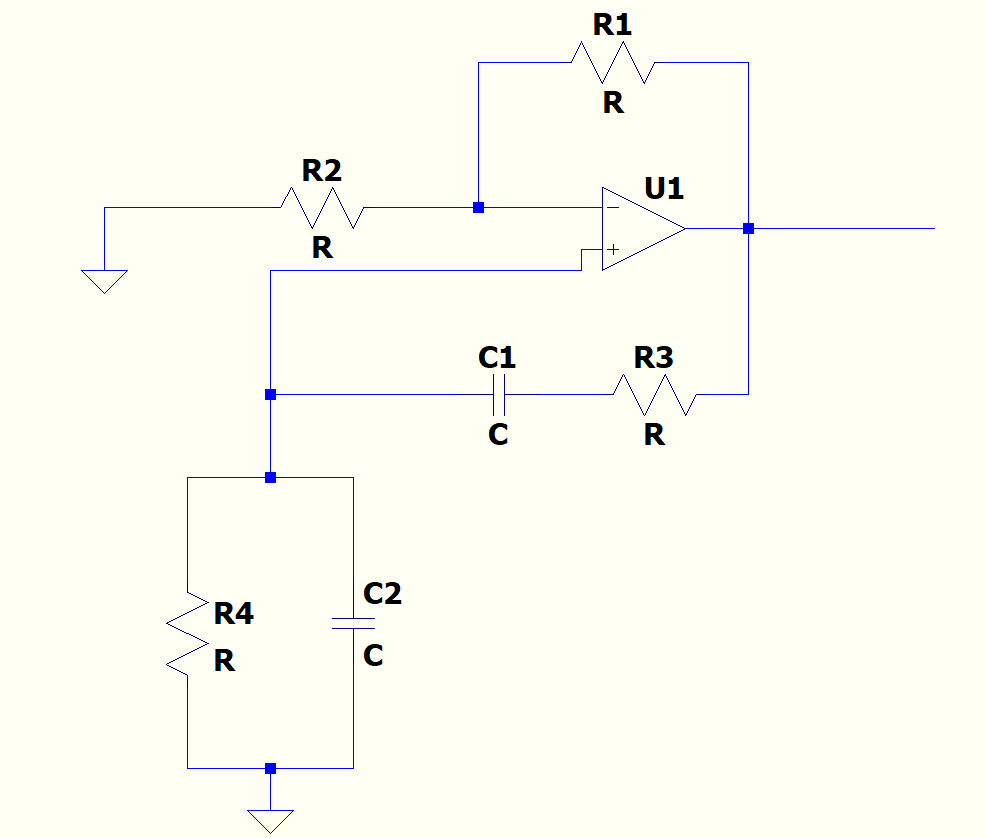
\includegraphics[width=0.6\linewidth]{fig/wien-bridge-schem.png}
    \caption{Wien Bridge Oscillator}
    \label{fig:wien_bridge}
\end{figure}




The positive feedback network is responsible for the resonant frequency setup and oscillation whereas the negative feedback network is responsible for the amplification.

In the positive feedback network, two RC networks one in series and the other in parallel are connected in series in the positive feedback network. The two RC networks are a low pass filter and a high pass filter which collectively acts as a notch pass filter so only a certain frequency is passed through it (Resonance Frequency).

In \Cref{fig:wien_bridge}, we take
\[
  R_3 = R_4 = R, \quad C_1 = C_2 = C
\]
Calculating the impedance of the circuit components,
$$Z_{R3} = Z_{R4} = R$$
$$Z_{C1} = Z_{C2} = \frac{1}{sC}$$

Resistor and capacitor connected in series forms the High Pass Filter,
$$Z_{HPF} = R + \frac{1}{sC}$$

Resistor and capacitor connected in parallel forms the low pass filter.
$$Z_{LPF} = \frac{1}{\frac{1}{R} + sC}$$

Voltage divider at non inverting input
$$V_+ = \frac{Z_{LPF}}{Z_{LPF} + Z_{HPF}} V_{out}$$
$$V_+ = \frac{\frac{1}{\frac{1}{R} + sC}}{R + \frac{1}{sC} + \frac{1}{\frac{1}{R} + sC}} V_{out}$$
simplifies into
$$V_+ = \frac{R}{R + \frac{(1 + sRC)^2}{sC}} V_{out}$$


 $$s = j \omega $$
$$\therefore V_+ = \frac{R}{R + \frac{(1 + j \omega RC)^2}{j \omega C}} V_{out}$$

\begin{equation}
\boxed{V_+ = \frac{R}{R + \frac{(1 + j \omega RC)^2}{j \omega C}} V_{out}}
\label{eqn. 1}
\end{equation}


For the negative feedback network,
\begin{equation}
    \boxed{V_{out} = (1 + \frac{R_1}{R_2})V_+}
    \label{eqn. 2}
\end{equation}

using \cref{eqn. 1} and \cref{eqn. 2},

$$V_{\text{out}} = \left(1 + \frac{R_1}{R_5}\right) V_+ 
= (1 + \frac{R_1}{R_2}) \frac{R}{R + \frac{(1 + j\omega R C)^2}{jC\omega}} V_{out}$$

$$\implies 1 = (1 + \frac{R_1}{R_2})\frac{R}{R + \frac{(1 + j\omega R C)^2}{jC\omega}}$$

for $\frac{(1 + j\omega R C)^2}{jC\omega}$ to be real,

$$\angle(jC\omega) = 90^\circ$$
$\therefore$ we want the numerator also to be in $90^\circ$
$$\implies \angle(1 + jRC\omega)^2 = 90^\circ$$
$$\implies Re\{(1 + jCR\omega )\} = Im\{(1 + jCR\omega)\}$$
$$\implies 1 = CR\omega$$
$$\therefore \omega = \frac{1}{RC}$$
\begin{equation}
    \omega = \frac{1}{RC}
    \label{eqn.3}
\end{equation}

therefore, the resonant frequency becomes,
$$\boxed{f_r = \frac{1}{2\pi R C}}$$
from \cref{eqn.3},\\
\\
 \[
\text{Loop gain}= \left(1 + \frac{R_1}{R_2} \right) \cdot \frac{R}{R + R\frac{(1 + j)^2}{j}}
\]
$$\implies \text{Loop Gain} = {\left(1 + \frac{R_1}{R_2}\right)}\frac{1}{1 + \frac{2j}{j}}$$
$$\implies \text{Loop gain} = \left(1 + \frac{R_1}{R_2}\right)\frac{1}{3}$$
\\
To sustain oscillations, Loop gain = 1
$$\boxed{\therefore \frac{R_1}{R_2} = 2}$$

The Amplitude of the oscillations is determined by the dynamically regulated non linear feedback mechanism that adjusts the gain to maintain steady oscillations.

We are tasked to make a quadrature oscillator that produces a sine wave of frequency of 100 KHz and amplitude of $1V_{pp}$. The sine wave should oscillate between $+0.5V_{pp}$ and $-0.5V_{pp}$.\\

Selecting a standard value for $C = 1 \text{nF}$\\
so, $R$ should be $R \approx 1.59\text{ K}\Omega$

For $ R = 1.6 \text{K}\Omega$ and $C = 1\text{nF}$, $f_r \approx 100\text{KHz}$.

And $\frac{R_1}{R_2} = 2$, so we take $R_1 = 20 K\Omega$ and $R_2 = 10 K\Omega$.\\
\\
Theoretical values are calculated.\\
When put these values to simulation, the frequency of the oscillation was approx. 50KHz, which is half the frequency we need. After fine tuning the components to arrive at a frequency of $100KHz$, the components take up the following values:

$$R = 900\Omega$$
$$C = 0.9nF$$
$$R_1 = 25K\Omega$$
$$R_2 = 10K\Omega$$

This gives the oscillation of frequency 100KHz and amplitude 710 mV. To adjust the amplitude to 500mV, we use a voltage divider to control it.

\begin{figure}[H]
    \centering
    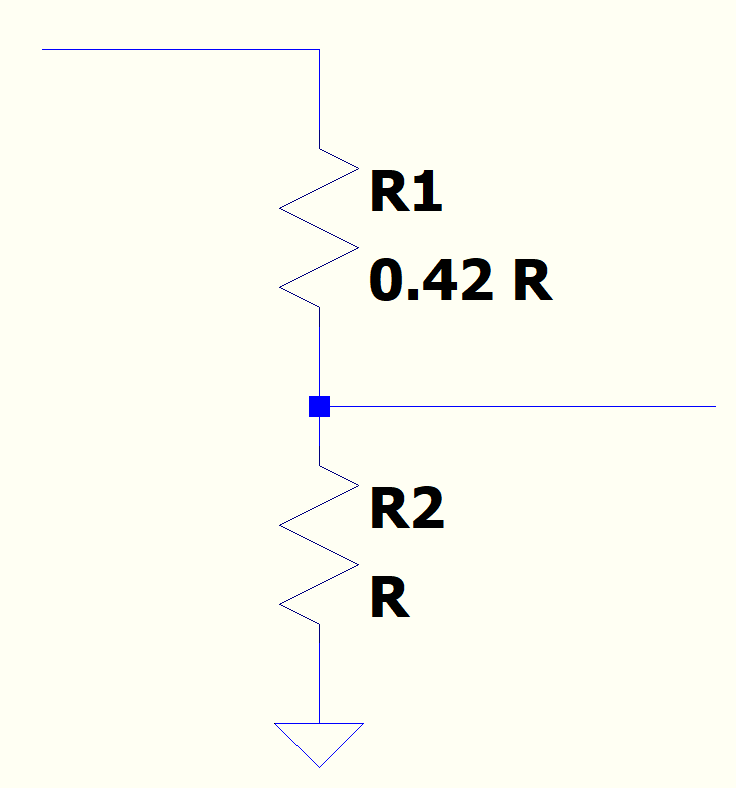
\includegraphics[width=0.6\linewidth]{Voltage-divider.png}
    \caption{Voltage Divider}
    \label{fig:voltage-div}
\end{figure}

In the Voltage divider,
$$V_{out} = V_{in}\cdot \frac{R_2}{R_1 + R_2}$$
$$\implies 500\text{ mV} = 710 \text{ mV} \cdot \frac{R_2}{R_1 + R_2}$$
$$\implies 0.704 = \frac{R_2}{R_1 + R_2}$$
$$\implies \frac{R_1}{R_2} = \frac{1}{0.704} - 1 \approx 0.42$$

Taking standard values, $R_2 = 10K\Omega$ and $R_1 = 4.2K\Omega$.
In the simulation, we got a value of 524 mV from the voltage divider. After fine tuning the values to achieve 500 mV, the values arrived at are,
$$R_1 = 5.1K\Omega$$
$$R_2 = 10k\Omega$$

We take one output from this voltage divider, this will be our In-phase component of the quadrature oscillator.\\
We take this signal to phase shift it by $90^\circ$, 

\begin{figure}[H]
    \centering
    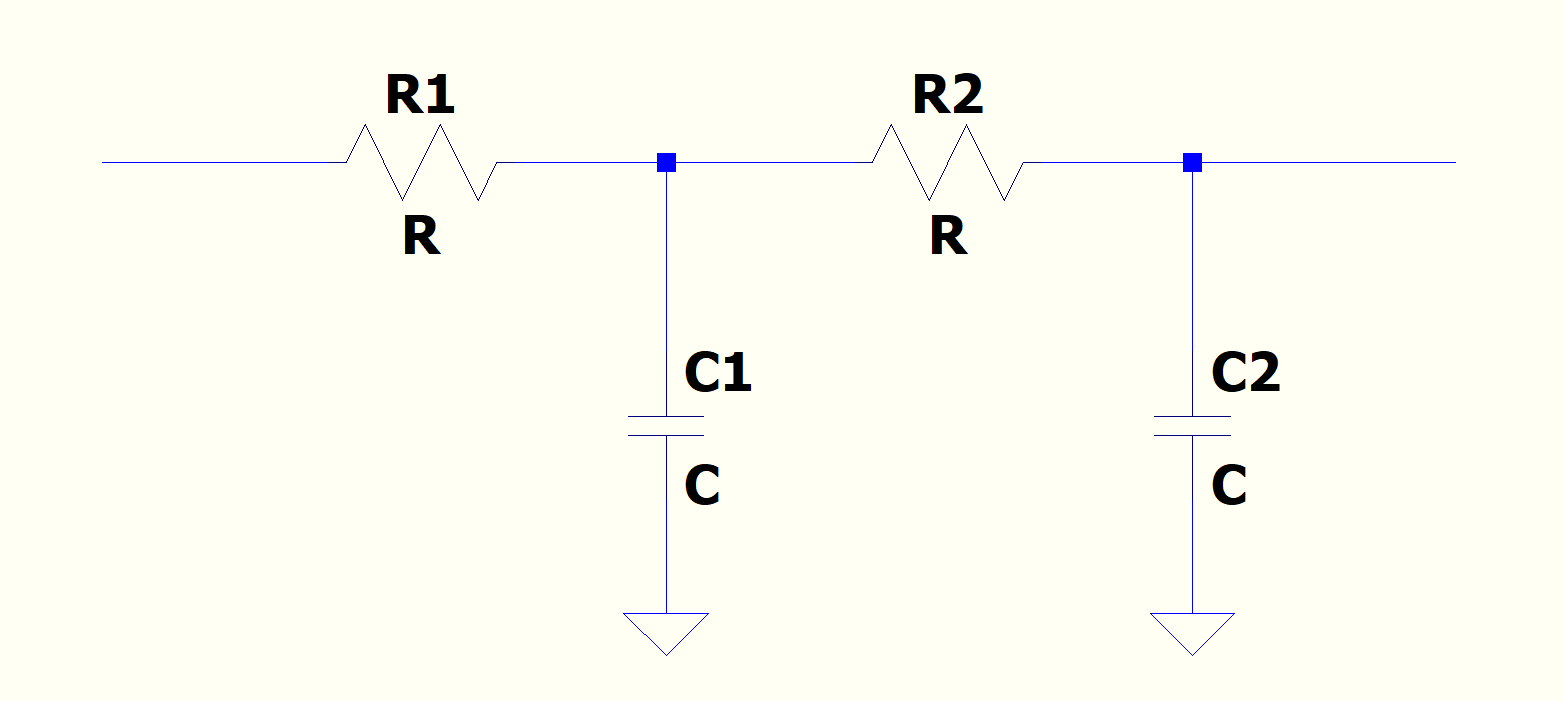
\includegraphics[width=0.8\linewidth]{Phase-shift.png}
    \caption{Phase Shifter}
    \label{fig:phase-shift}
\end{figure}

There are 2 RC stages in this circuit block (refer to \cref{fig:phase-shift}). Each RC stage provides a phase shift of $45^\circ$ which gives a total phase shift of $90^\circ$.
\\
\\
For each RC stage, transfer function of the stage is
$$H(\omega) = \frac{1}{ 1 + j\omega RC}$$\\
The phase shift of this stage is 
$$\phi(\omega) = -\tan^{-1}(\omega RC)$$
This is a lagging phase shift, for two stages
$$\phi_{tota} = 2 \cdot \phi = -90^\circ \implies \phi = -45^\circ \text{ per stage}$$
To solve for RC at $45^\circ$
$$\tan^{-1}(\omega RC) = \frac{\pi}{4} \implies \omega RC = \tan(\frac{\pi}{4}) = 1$$
we substitute, $\omega = 2\pi f = 2\pi \cdot 10^5 rad/s$
$$RC = \frac{1}{\omega} = \frac{1}{2\pi \cdot 10^5} = 1.595 \times 10^{-6}s$$
For standard values,
$$R = 1.6K\Omega$$
$$C = 1nF$$

When simulated with the theoretical values, the time difference between two peaks of the two waves comes out to be $2.2 \mu s$ which give the phase shift by approximately $-109^\circ$. After fine tuning the values, for phase shift by $-90^\circ$, the time difference between the two wave peaks should be equal to $2.5 \mu s$.
$$T = \frac{1}{f} \text{(Period of the wave)}$$
Phase shift by $90^\circ$ means $\Delta t = \frac{T}{4}$
$$\implies T = \frac{1}{100000} = 10 \mu s$$
$$\implies \Delta t = \frac{10 \mu s}{4} = 2.5 \mu s$$

The values of the components after fine tuning comes as,
$$R = 1K\Omega$$
$$C = 0.93nF$$

This also attenuates the amplitude of the wave to 256 mV.
To maintain the amplitude of the phase shifted wave at 500 mV, we use an op-amp amplifier to do the same.
\begin{figure}[H]
    \centering
    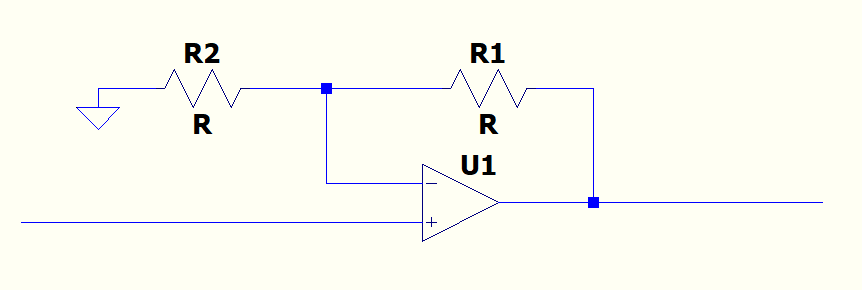
\includegraphics[width=0.75\linewidth]{op-amp-amplifier.png}
    \caption{Op-amp inverting Amplifier}
    \label{fig:op-amp-amp}
\end{figure}

$\because$ the phase shift from the RC Phase shift circuit is $-90^\circ$, we can use an inverting amplifier so that the total phase shift becomes $180^\circ - 90^\circ = 90^\circ$.

This converts the lagging phase shift into leading phase shift.\\
\\
We know,

$$\text{Gain } = \frac{V_{out}}{V_{in}} = \frac{500mV}{256mV} \approx 1.95$$

$\because$ the circuit is an inverting amplifier, we know
$$A_v = -\frac{R_1}{R_2}$$
as we are inverting the signal, we ignore the negative sign for calculations.

$$1.95 = \frac{R_1}{R_2}$$
Taking standard value for $R_2 = 10K\Omega$, we get $R_1 = 40.65K\Omega$
$$R_1 = 19.53K\Omega$$
$$R_2 = 10K\Omega$$

When simulated with the theoretical values, the amplitude of the phase shifted wave was approx. 760m V. When fine tuned the component values for amplitude 500 mV, we get the following values,
$$R_1 = 8.4K\Omega$$
$$R_2 = 8.9K\Omega$$

Now, we have the amplitude of the phase shifted wave is 500 mV. The output of this inverting amplifier, is our quadrature component of the oscillator.\\
\\
To make sure that none of the impedance of the different circuit blocks affect the achieved signal, we use a voltage buffer between the circuit blocks (\cref{fig:op-amp-buffer}).
\begin{figure}[H]
    \centering
    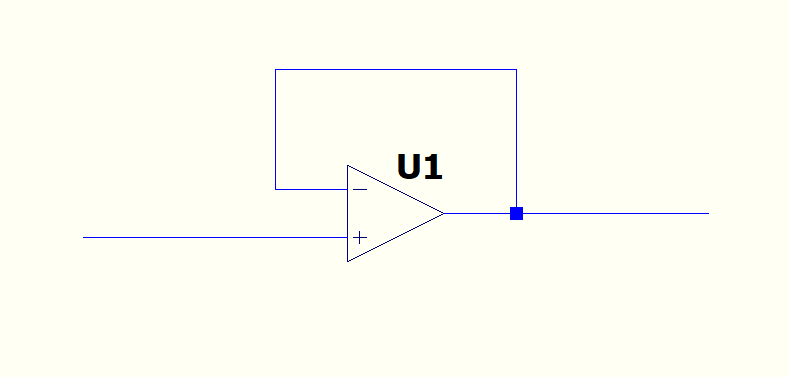
\includegraphics[width=1\linewidth]{voltage-buffer.png}
    \caption{Op-amp Voltage Buffer}
    \label{fig:op-amp-buffer}
\end{figure}
We are now done with the design of our quadrature oscillator.

\begin{figure}[H]
    \centering
    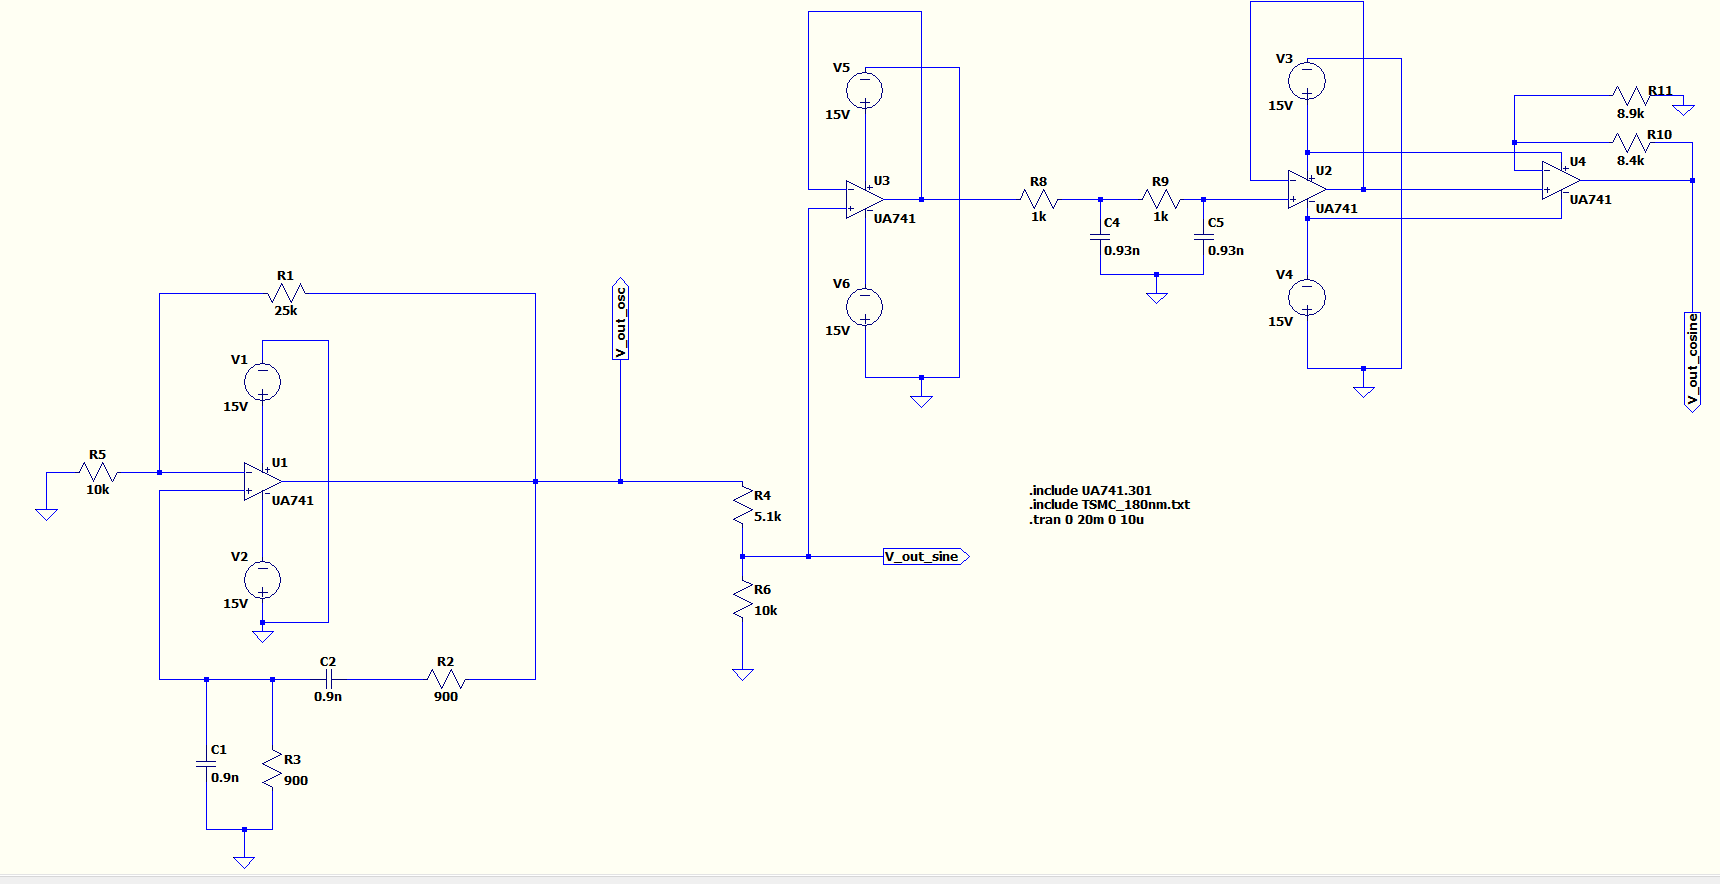
\includegraphics[width=1\linewidth]{quad-osc-ckt.png}
    \caption{Quadrature Oscillator Circuit}
    \label{fig:enter-label}
\end{figure}

\subsection{Simulation and results.}
\begin{figure}[H]
    \centering
    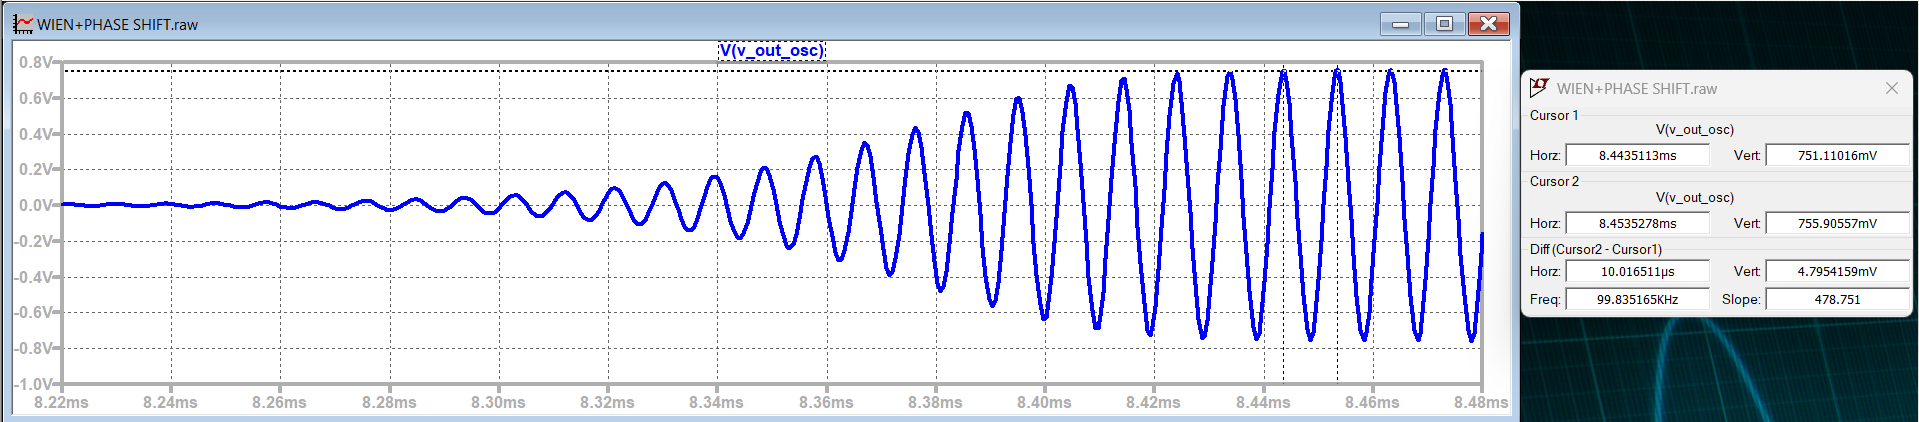
\includegraphics[width=1\linewidth]{wien-osc-output.png}
    \caption{Output signal of the Wien-bridge oscillator}
    \label{fig: wien-output}
\end{figure}

Frequency of the wave is $\approx 100 KHz$ and amplitude is $\approx 750mV$.\\
To adjust the amplitude, we used a voltage divider.
\begin{figure}[H]
    \centering
    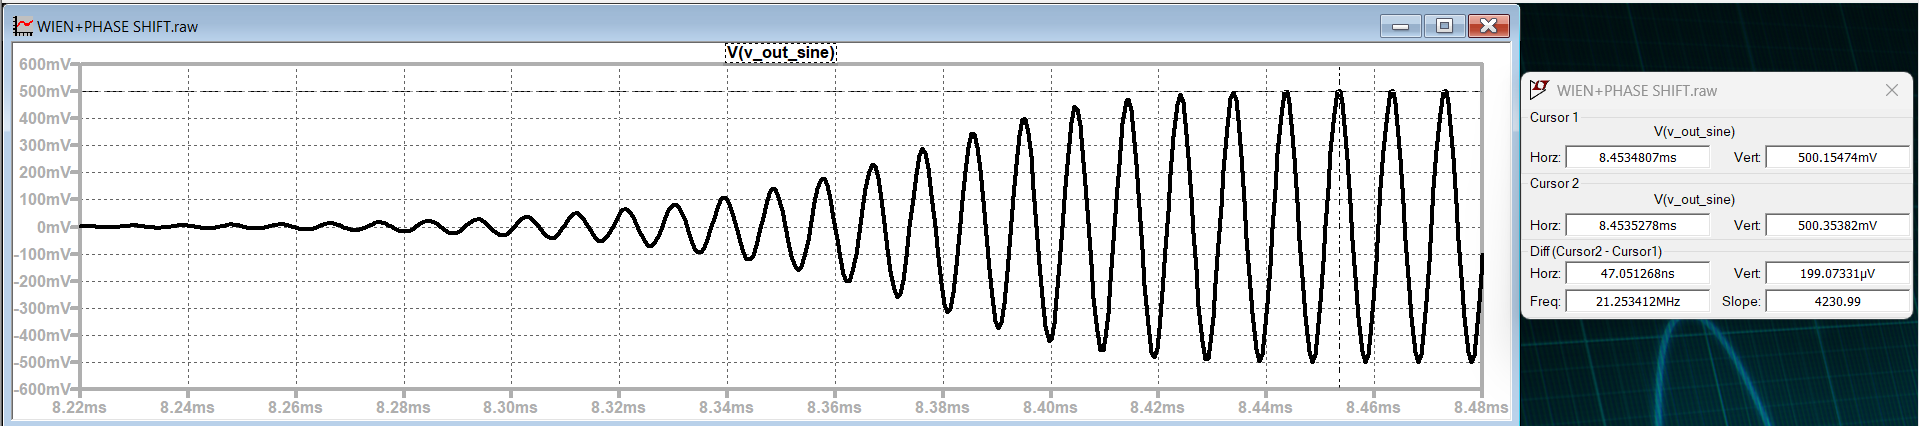
\includegraphics[width=1\linewidth]{voltage-div-output.png}
    \caption{Output signal of the voltage divider.}
    \label{fig:enter-label}
\end{figure}

Amplitude of the sine wave is now set at 500 mV, this is our in-phase component of the signal. For quadrature component, we phase shifted it using the RC Phase shift circuit.
\begin{figure}[H]
    \centering
    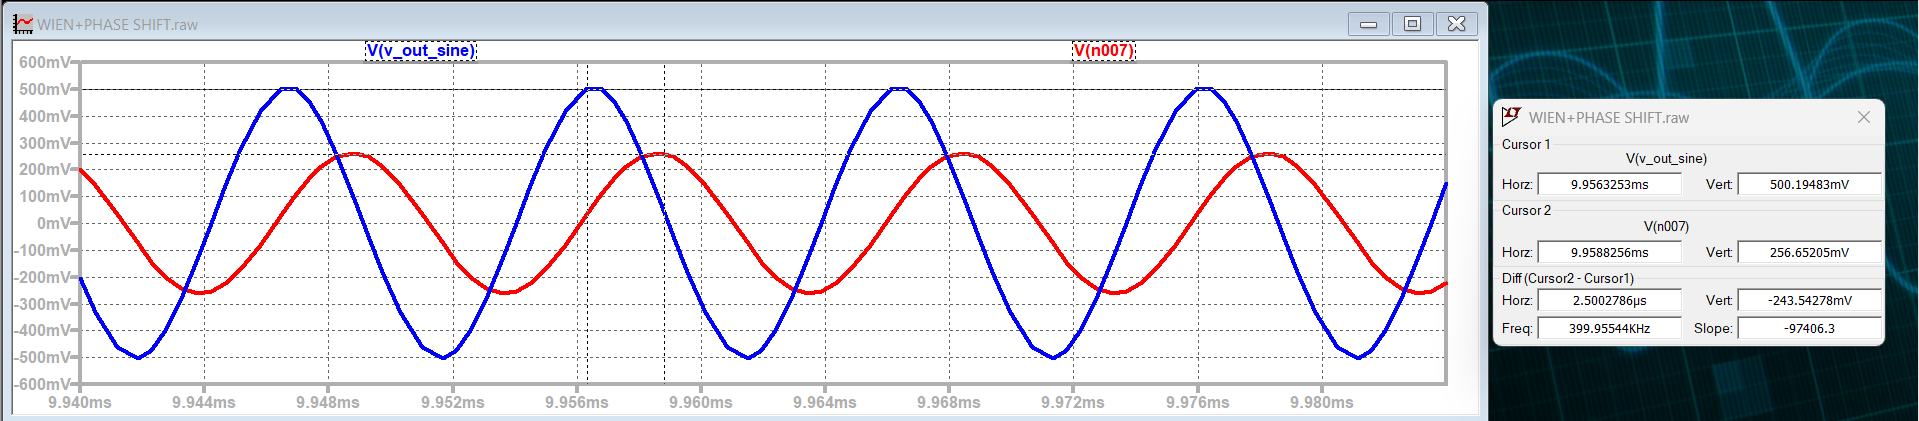
\includegraphics[width=1\linewidth]{RC-phase-shift-output.png}
    \caption{Output signal of the RC Phase shift circuit}
    \label{fig:rc-phase-shift-output}
\end{figure}
As you can see the time difference between the two peaks of the waves is $2.5 \mu s$ which is what we calculated earlier. The wave is phase shifted by $90^\circ$.\\
We used an inverting op-amp amplifier to maintain the amplitude of the quadrature component at 500 mV.
\begin{figure}[H]
    \centering
    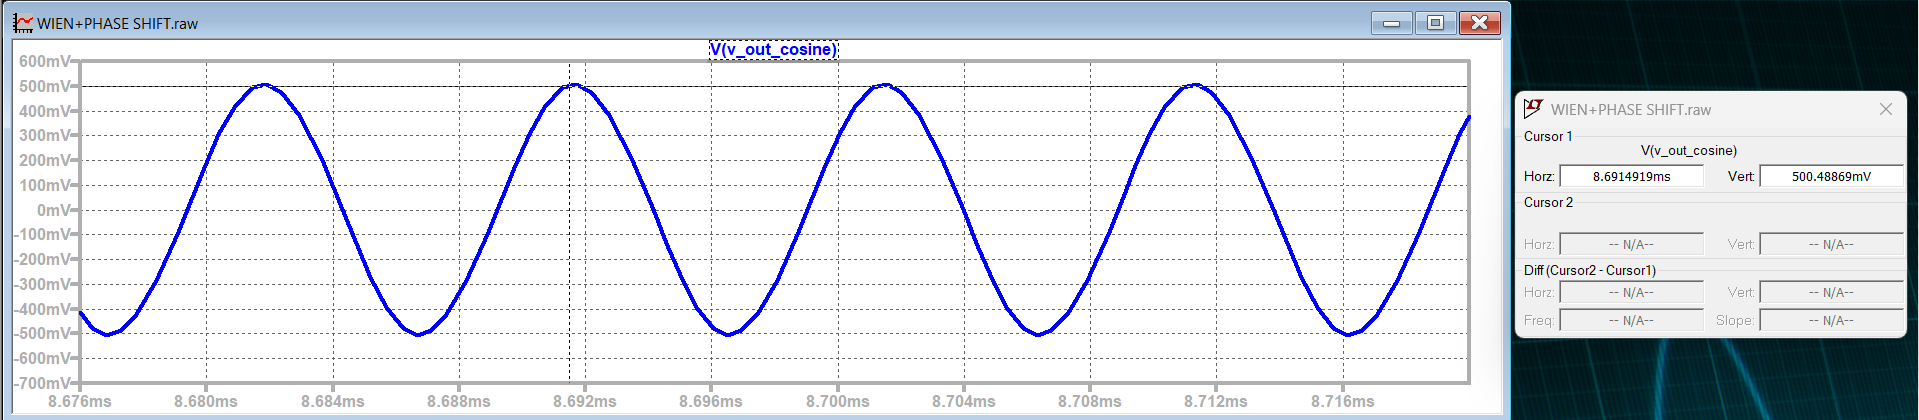
\includegraphics[width=1\linewidth]{op-amp-amp-output.png}
    \caption{Output signal of the Inverting op-amp amplifier}
    \label{fig:enter-label}
\end{figure}

This is our quadrature component of the oscillator.\\
\\
The final result of the simulation is as follows:
\begin{figure}[H]
    \centering
    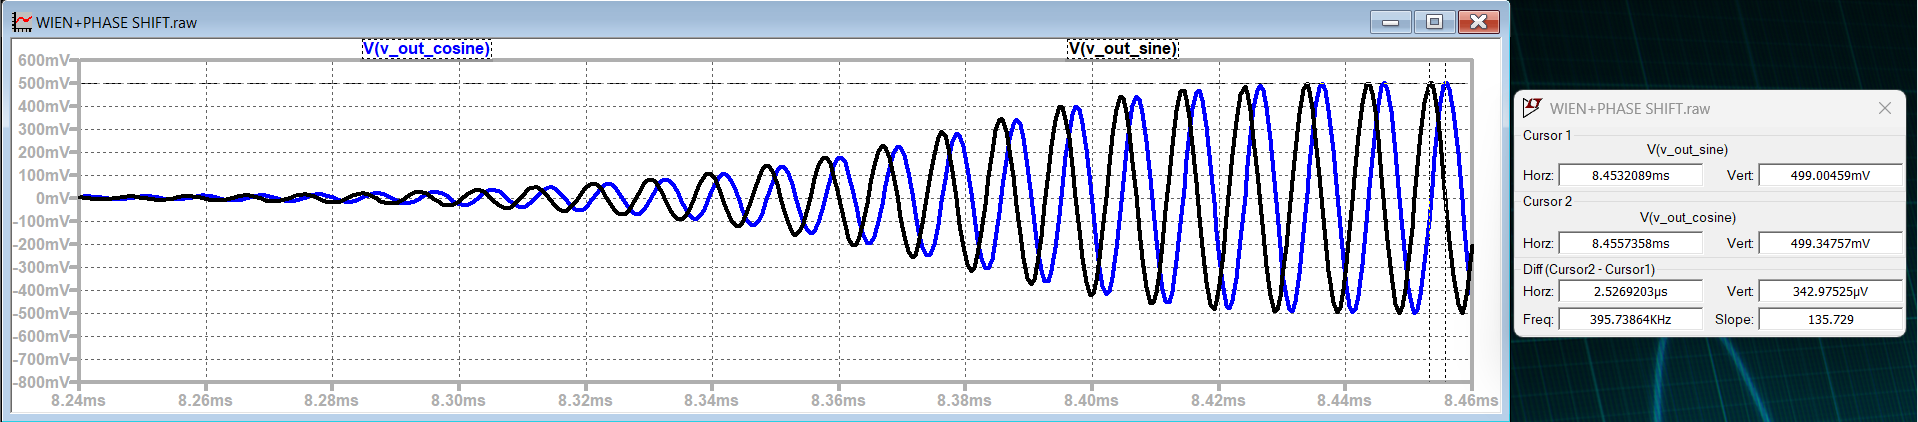
\includegraphics[width=1\linewidth]{Final-simulation-result.png}
    \caption{Final simulation Result}
    \label{fig:enter-label}
\end{figure}

As shown in the result the amplitude of the in-phase component of the signal (V\_out\_sine) and quadrature component of the signal (V\_out\_cosine) is $\approx 500 mV$ and the time difference between two simultaneous peaks of the wave is $\approx 2.5 \mu s$, which concludes that the phase difference between the two waves is $90^\circ$.\\
\\
This is our desired quadrature oscillator.

\section{The Mixer}
\label{sec:mixer}
\subsection{Ideation, Formulation and Analysis}

The mixer is a fundamental building block in our quadrature down converter, responsible for frequency translation by multiplying the input signal with the local oscillator (LO) signal. In this project, we implement a simple NMOS-based switching mixer, as shown in Fig.~\ref{fig:nmos_mixer}.

\begin{figure}[H]
    \centering
    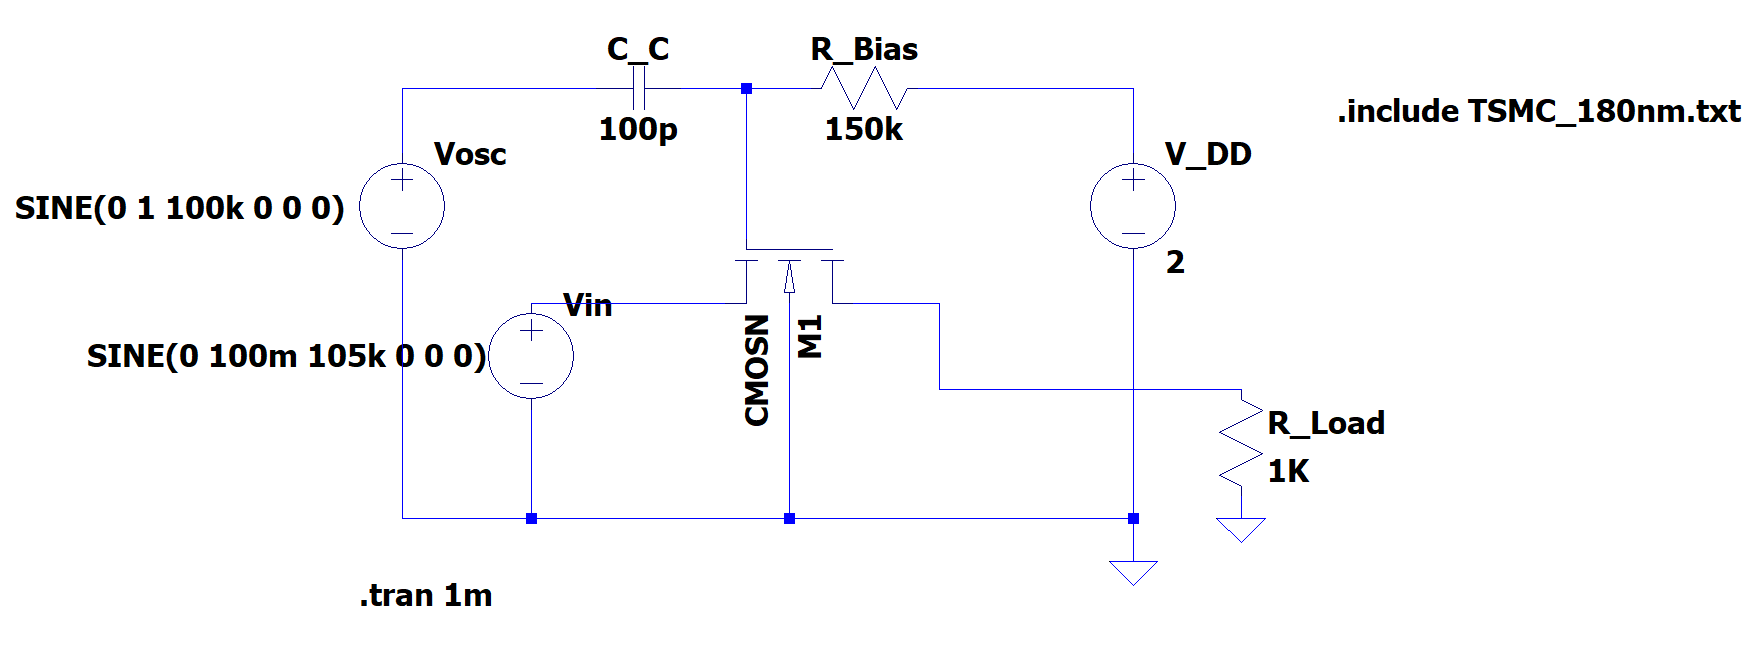
\includegraphics[width=\linewidth]{fig/mixer.png}
    \caption{NMOS Mixer Schematic (LTspice)}
    \label{fig:nmos_mixer}
\end{figure}

\subsubsection{Circuit Configuration}
The mixer consists of:
\begin{itemize}
    \item \textbf{NMOS transistor (M1)}: TSMC 180nm model, acts as the mixing element
    \item \textbf{Coupling capacitor ($C_C = 100$ pF)}: Blocks DC while passing AC oscillator signal
    \item \textbf{Bias resistor ($R_{Bias} = 150$ k$\Omega$)}: Provides DC path for proper gate biasing
    \item \textbf{Load resistor ($R_L = 1$ k$\Omega$)}: Converts drain current to output voltage
    \item \textbf{Input signal}: $V_{in} = 100$ mV amplitude at $(100 + \Delta f)$ kHz
    \item \textbf{Oscillator signal}: $V_{OSC} = 1$ V amplitude at 100 kHz
    \item \textbf{Supply voltage}: $V_{DD} = 2$ V
\end{itemize}
\subsubsection{Component Value Selection}
The component values were carefully chosen to ensure optimal mixer performance:

\begin{itemize}
    \item \textbf{Coupling Capacitor ($C_C = 100$ pF)}
    \begin{itemize}
        \item \textit{Purpose}: Blocks DC while passing AC oscillator signal to gate
        \item \textit{Selection rationale}: Provides low impedance ($\approx 15.9$ k$\Omega$) at 100 kHz
        \item \textit{Desired range}: 10 pF - 1 nF
        \begin{itemize}
            \item Too small ($<$10 pF): High impedance limits signal coupling
            \item Too large ($>$1 nF): Unnecessary physical size, longer discharge time
        \end{itemize}
    \end{itemize}
    
    \item \textbf{Bias Resistor ($R_{Bias} = 150$ k$\Omega$)}
    \begin{itemize}
        \item \textit{Purpose}: Provides DC path to ground for gate biasing
        \item \textit{Selection rationale}: High enough to minimize loading effects on oscillator
        \item \textit{Desired range}: 10 k$\Omega$ - 1 M$\Omega$
        \begin{itemize}
            \item Too small ($<$10 k$\Omega$): Loads oscillator signal, wastes power
            \item Too large ($>$1 M$\Omega$): May cause biasing instability, noise susceptibility
        \end{itemize}
    \end{itemize}
    
    \item \textbf{Load Resistor ($R_L = 1$ k$\Omega$)}
    \begin{itemize}
        \item \textit{Purpose}: Converts drain current variations to voltage
        \item \textit{Selection rationale}: Project requirement, balances output signal level with power consumption
        \item \textit{Desired range}: 100 $\Omega$ - 10 k$\Omega$
        \begin{itemize}
            \item Too small ($<$100 $\Omega$): Excessive current, low output voltage swing
            \item Too large ($>$10 k$\Omega$): Reduced bandwidth due to parasitic capacitances
        \end{itemize}
    \end{itemize}
    
    \item \textbf{Supply Voltage ($V_{DD} = 2$ V)}
    \begin{itemize}
        \item \textit{Purpose}: Powers the circuit, provides headroom for transistor operation
        \item \textit{Selection rationale}: Sufficient for 180 nm CMOS technology
        \item \textit{Desired range}: 1.8 V - 3.3 V
        \begin{itemize}
            \item Too low ($<$1.8 V): Insufficient headroom for proper operation
            \item Too high ($>$3.3 V): Excessive power consumption, potential reliability issues
        \end{itemize}
    \end{itemize}
    
    \item \textbf{Signal Parameters}
    \begin{itemize}
        \item \textit{Input signal} (100 mV): Appropriate level for linear operation
        \begin{itemize}
            \item Range: 10 mV - 500 mV
        \end{itemize}
        \item \textit{Oscillator signal} (1 V): Sufficient amplitude to ensure complete switching
        \begin{itemize}
            \item Range: 0.5 V - 2 V
        \end{itemize}
    \end{itemize}
\end{itemize}

\textbf{Mixer Principle:}  
The NMOS transistor operates as a time-varying resistor, controlled by the LO at its gate. When $V_{GS} > V_{th}$ (positive LO half-cycle), the device enters the triode region, allowing the input signal to pass to the drain. When $V_{GS} < V_{th}$ (negative LO half-cycle), the device is in cutoff and blocks the signal, except for small contributions via parasitic capacitance.

Mixing is mathematically described as:
$$
V_{IF} = V_{in} \times V_{OSC} 
$$
$$V_{IF}= \frac{A_1 A_2}{2} \left[ \cos((\omega_{in} - \omega_{osc})t) + \cos((\omega_{in} + \omega_{osc})t) \right]$$
 
where $A_1$ and $A_2$ are the amplitudes of the input and LO signals.

The mixer in our quadrature down converter performs frequency down-conversion, taking the $(100 + \Delta f)$ kHz input signal and translating it to a $\Delta f$ kHz intermediate frequency by mixing with the 100 kHz local oscillator. This frequency difference is essential for further signal processing in wireless communication systems where high-frequency signals need to be converted to lower frequencies for efficient processing.

\subsection{Simulation and Results}

To verify the performance of our NMOS mixer design, we conducted extensive LTspice simulations using the TSMC 180nm transistor model. The circuit was implemented as shown in Fig.~\ref{fig:nmos_mixer} with the component values specified in the previous section.

\begin{figure}[H]
    \centering
    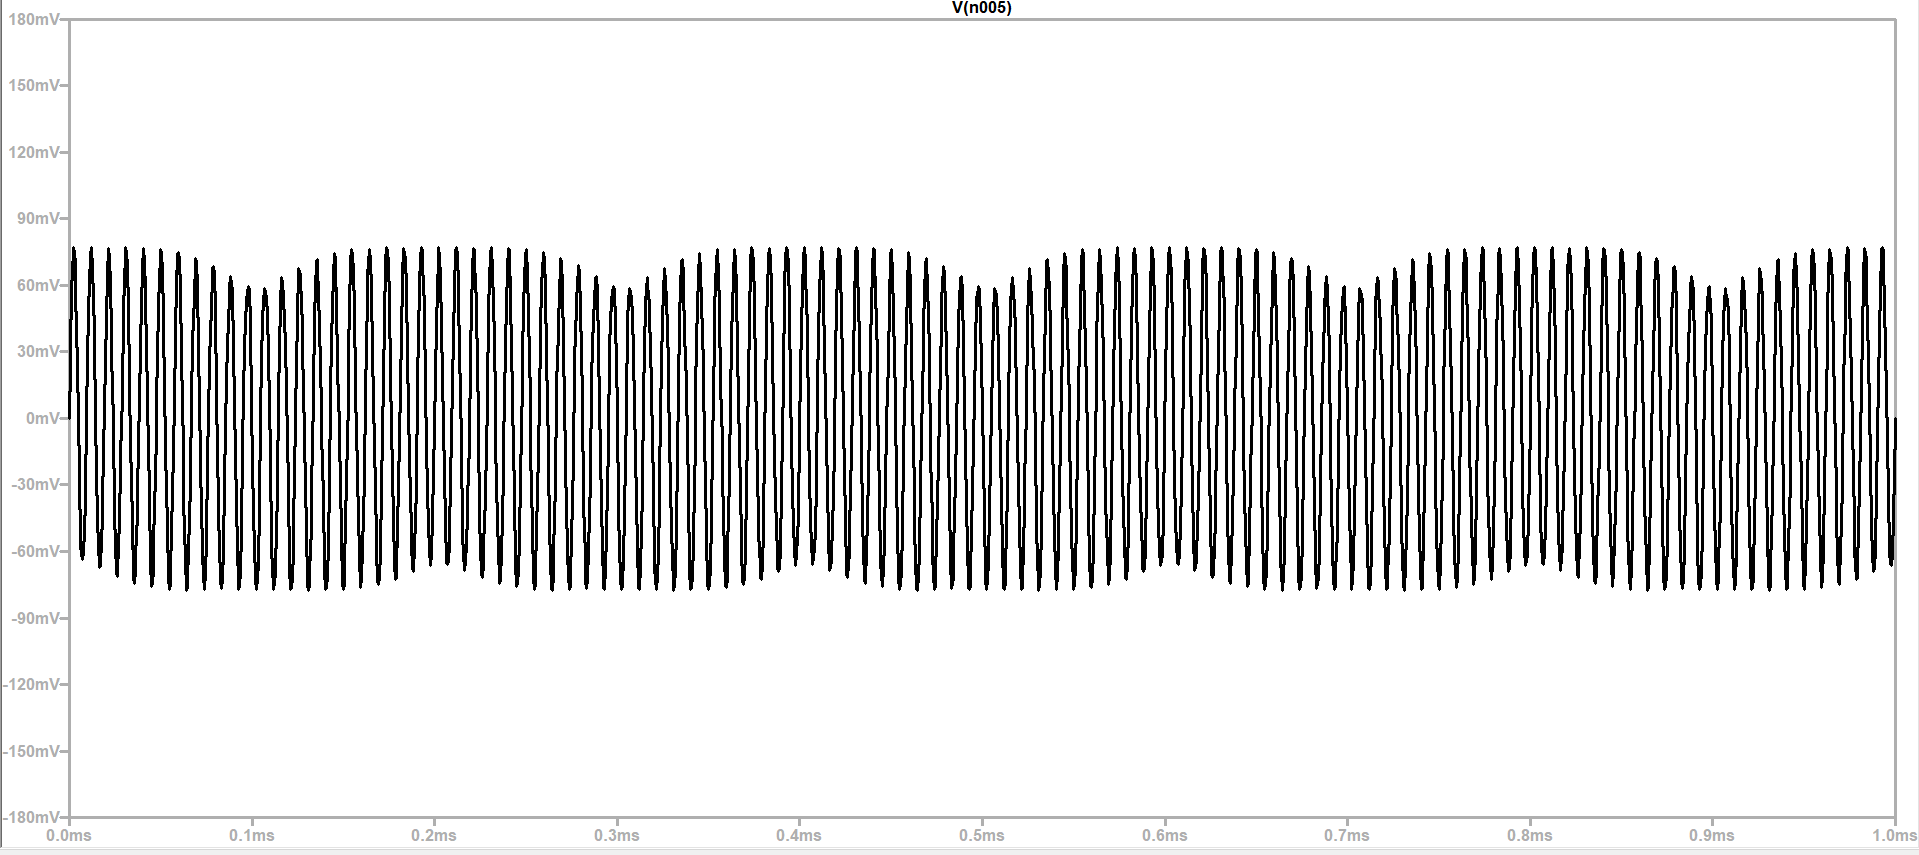
\includegraphics[width=\linewidth]{fig/105.png}
    \caption{Mixer Output Waveform ($V_{IF}$ at drain) for $f_{in} = 105$ kHz ($\Delta f = 5$ kHz)}
    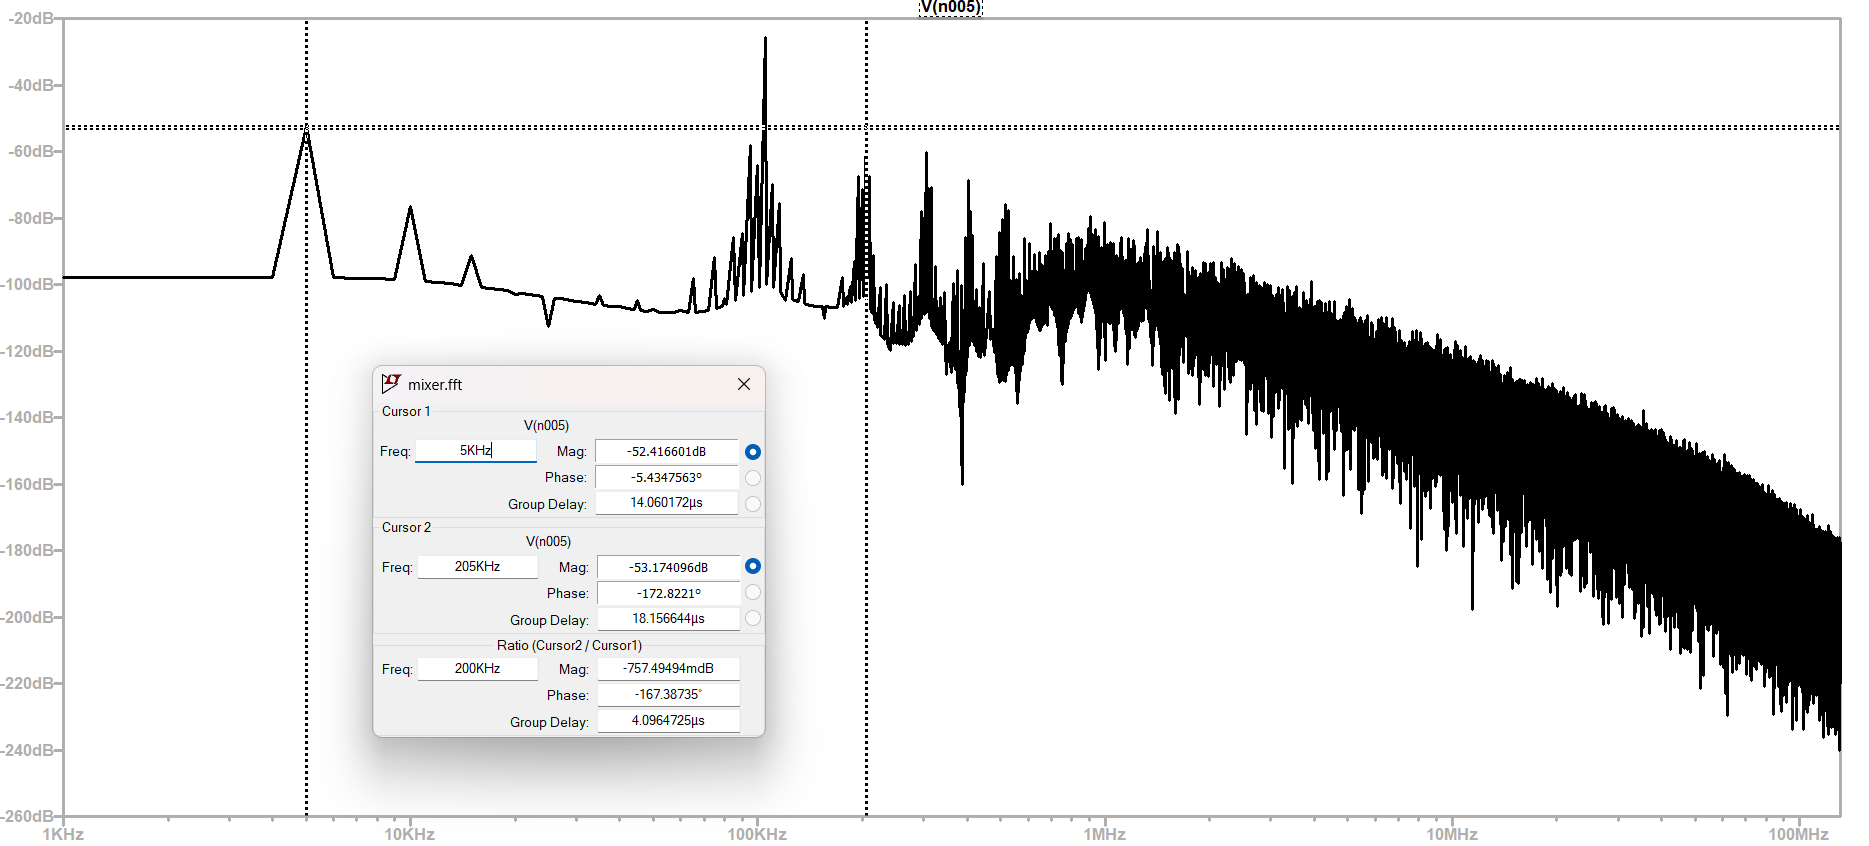
\includegraphics[width=1\linewidth]{fig/105fft.png}
     \caption{105kHz FFT}
    \label{fig:mixer_output}
\end{figure}

As seen in Fig.~\ref{fig:mixer_output}, the output waveform exhibits a clear beat pattern with an envelope frequency of $\Delta f = 5$ kHz, which corresponds to the difference between the input frequency (105 kHz) and the LO frequency (100 kHz). The output signal swings between approximately $-80$ mV and $+80$ mV, indicating a conversion gain of:

$$
G_c = \frac{V_{IF}}{V_{in}} \approx \frac{80\,\text{mV}}{100\,\text{mV}} = 0.8 \approx -1.94\,\text{dB}
$$

This conversion gain is typical for passive MOSFET mixers and demonstrates efficient frequency translation.

To thoroughly analyze the mixer's performance across various input frequencies, we conducted simulations with $f_{in} = \{95, 98, 99, 101, 102, 105\}$ kHz (corresponding to $\Delta f = \{5, 2, 1, 1, 2, 5\}$ kHz) while maintaining $f_{osc} = 100$ kHz. The results demonstrate the following behavior:

\begin{figure}[H]
    \centering
    % Place image of multiple frequency responses here
        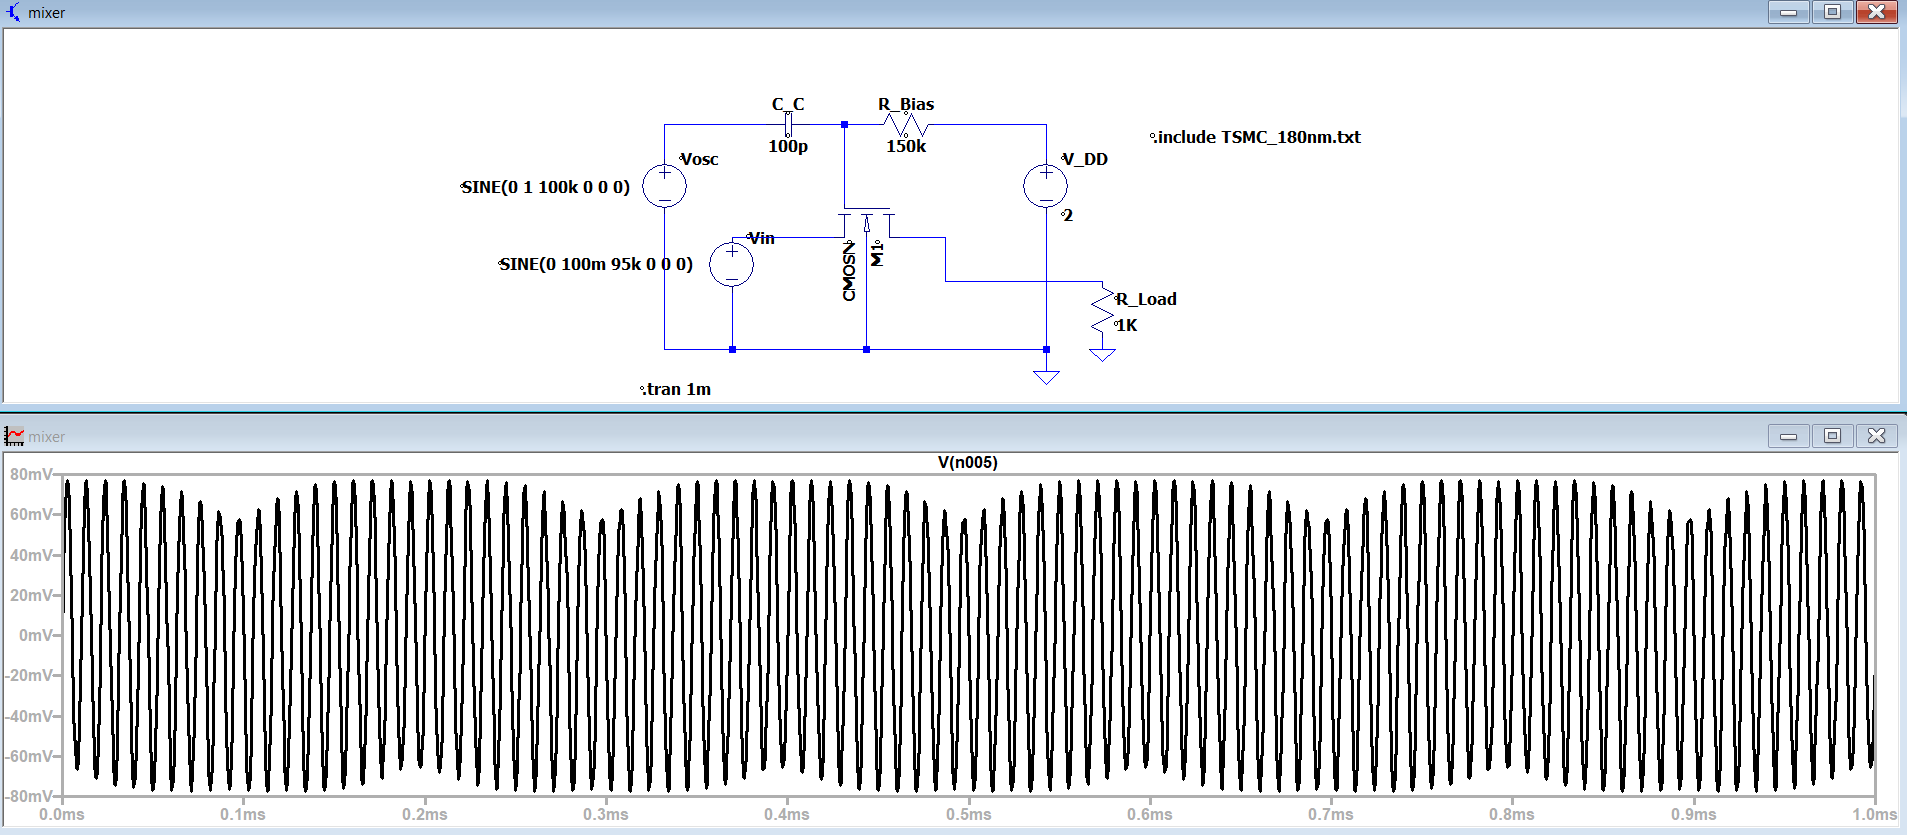
\includegraphics[width=1\linewidth]{fig/95.png}
        \caption{95kHz Output Signal}
         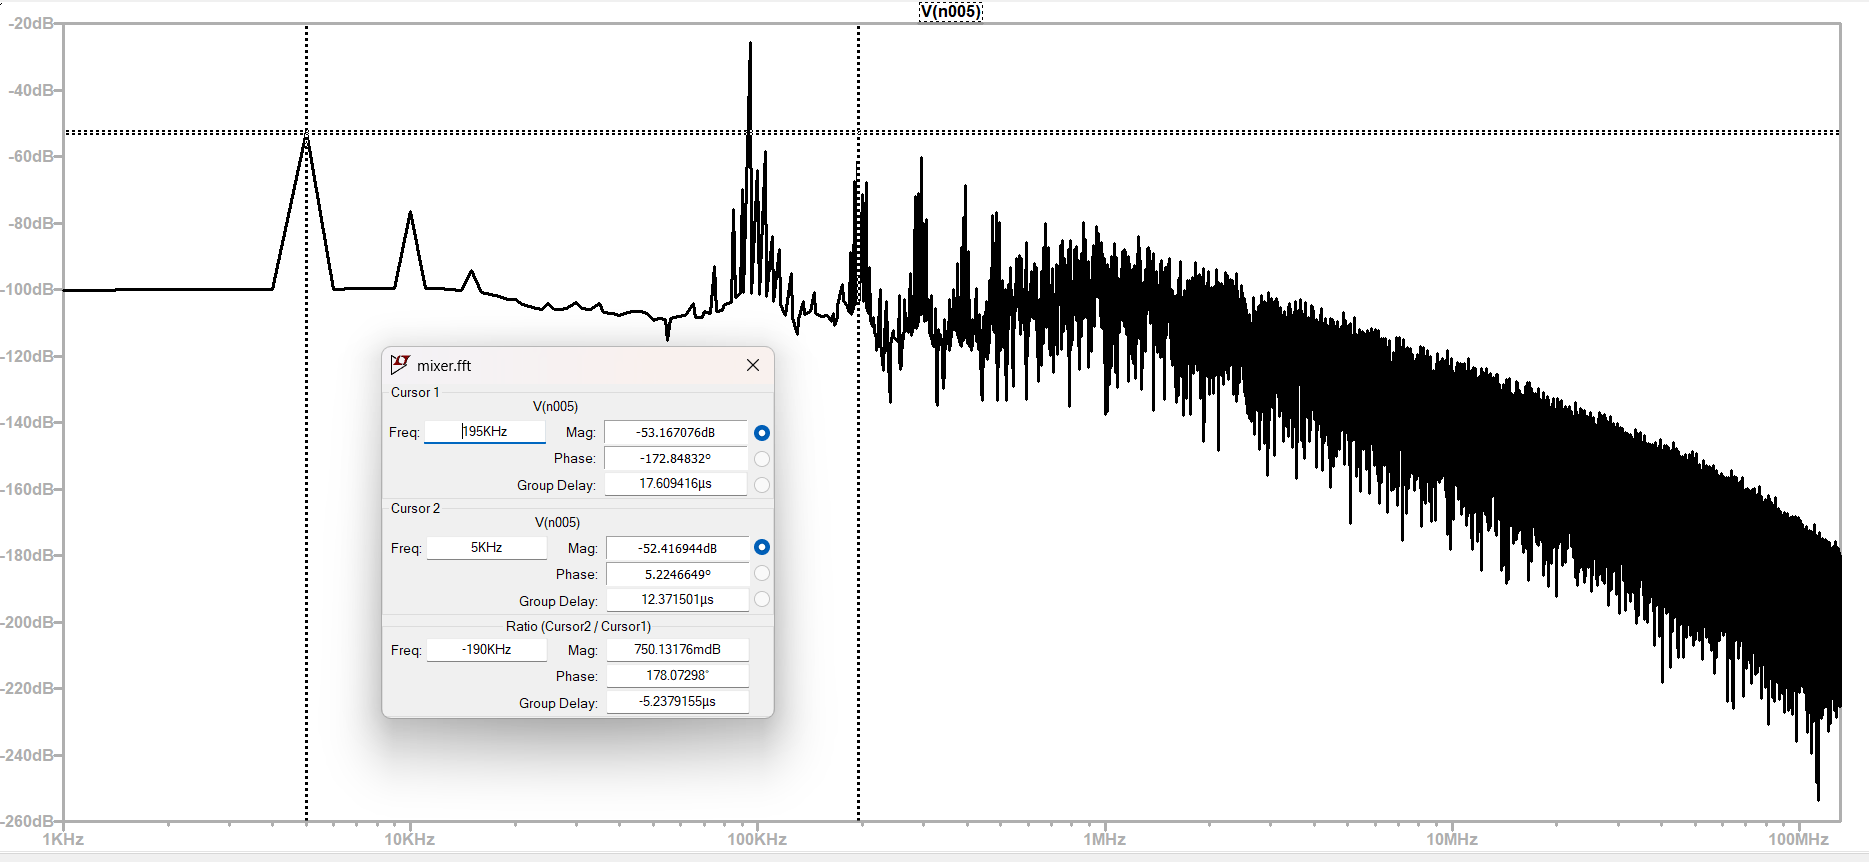
\includegraphics[width=1\linewidth]{fig/95fft.png}
        \caption{95kHz FFT}

\end{figure}
\begin{figure}
    \centering
    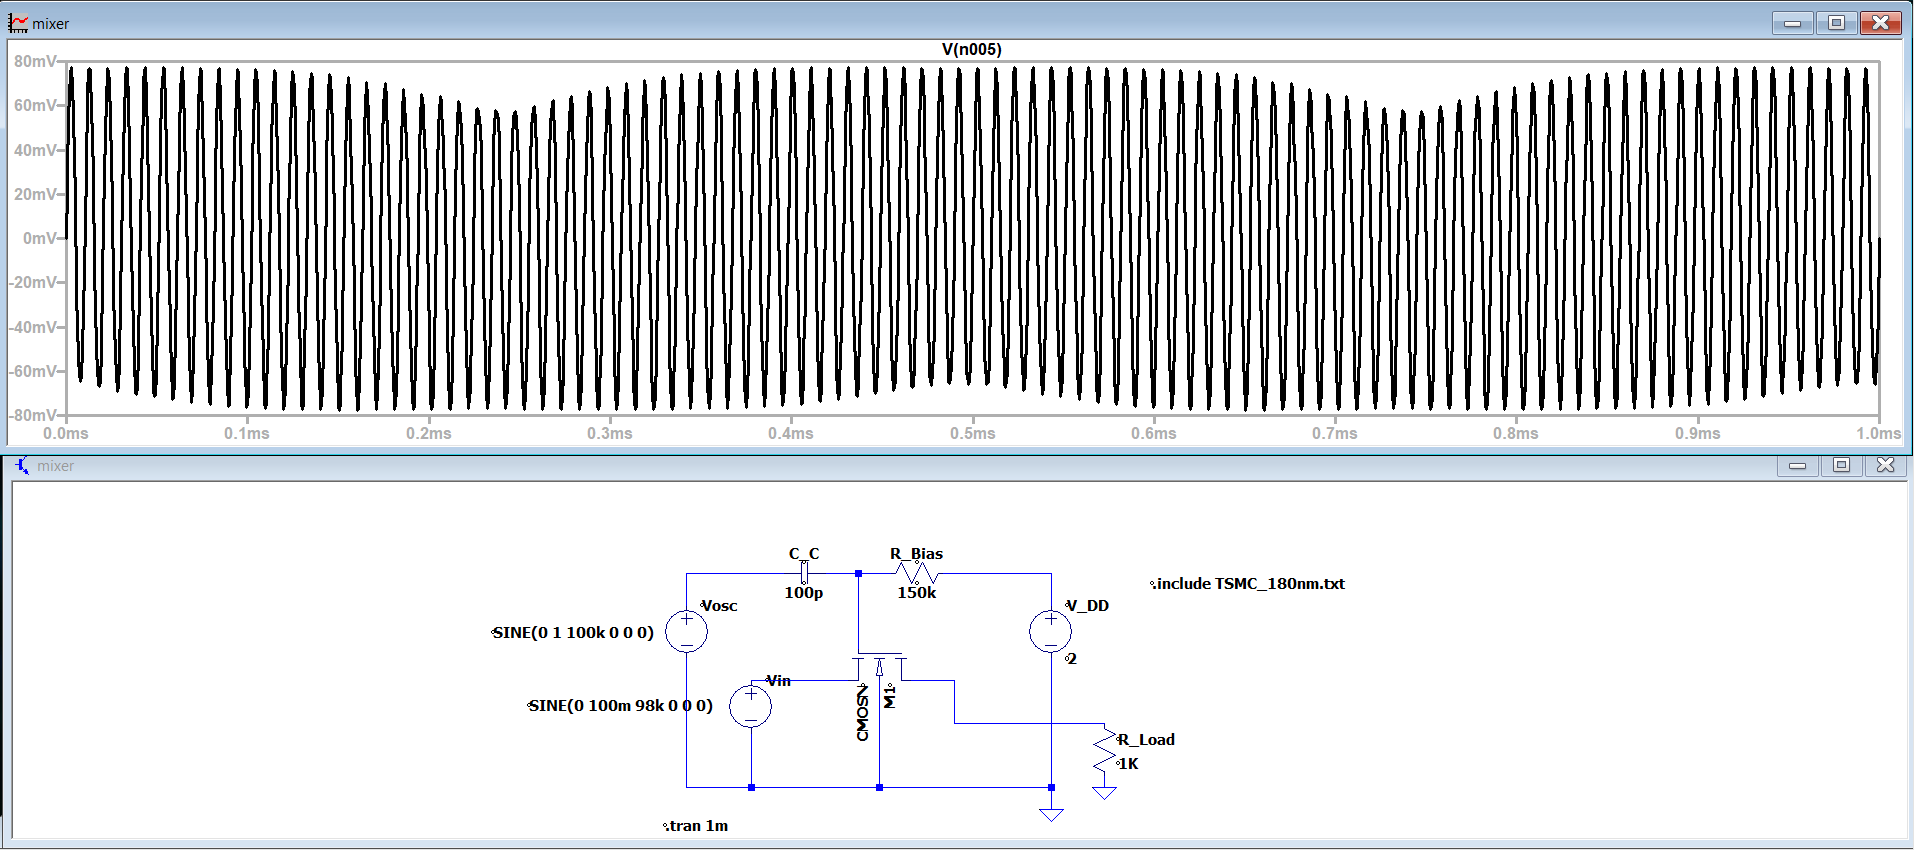
\includegraphics[width=1\linewidth]{fig/98.png}
    \caption{98kHz Output Signal}
    
    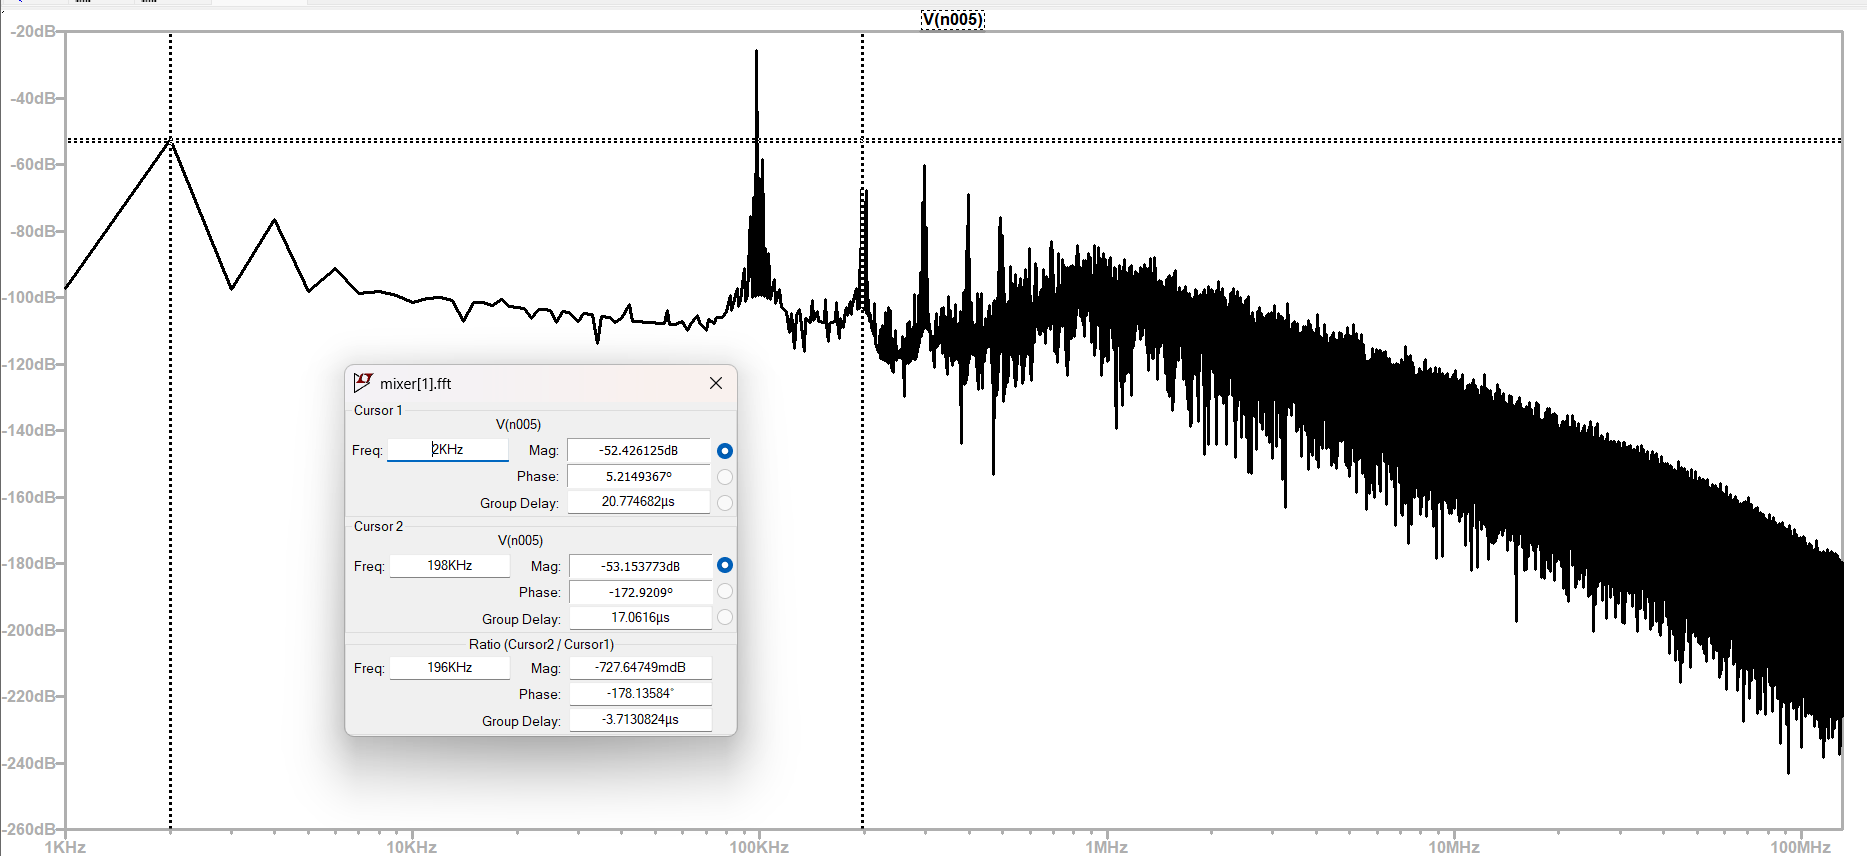
\includegraphics[width=1\linewidth]{98fft.png}
    \caption{98kHz FFT}
\end{figure}
\begin{figure}
    \centering
    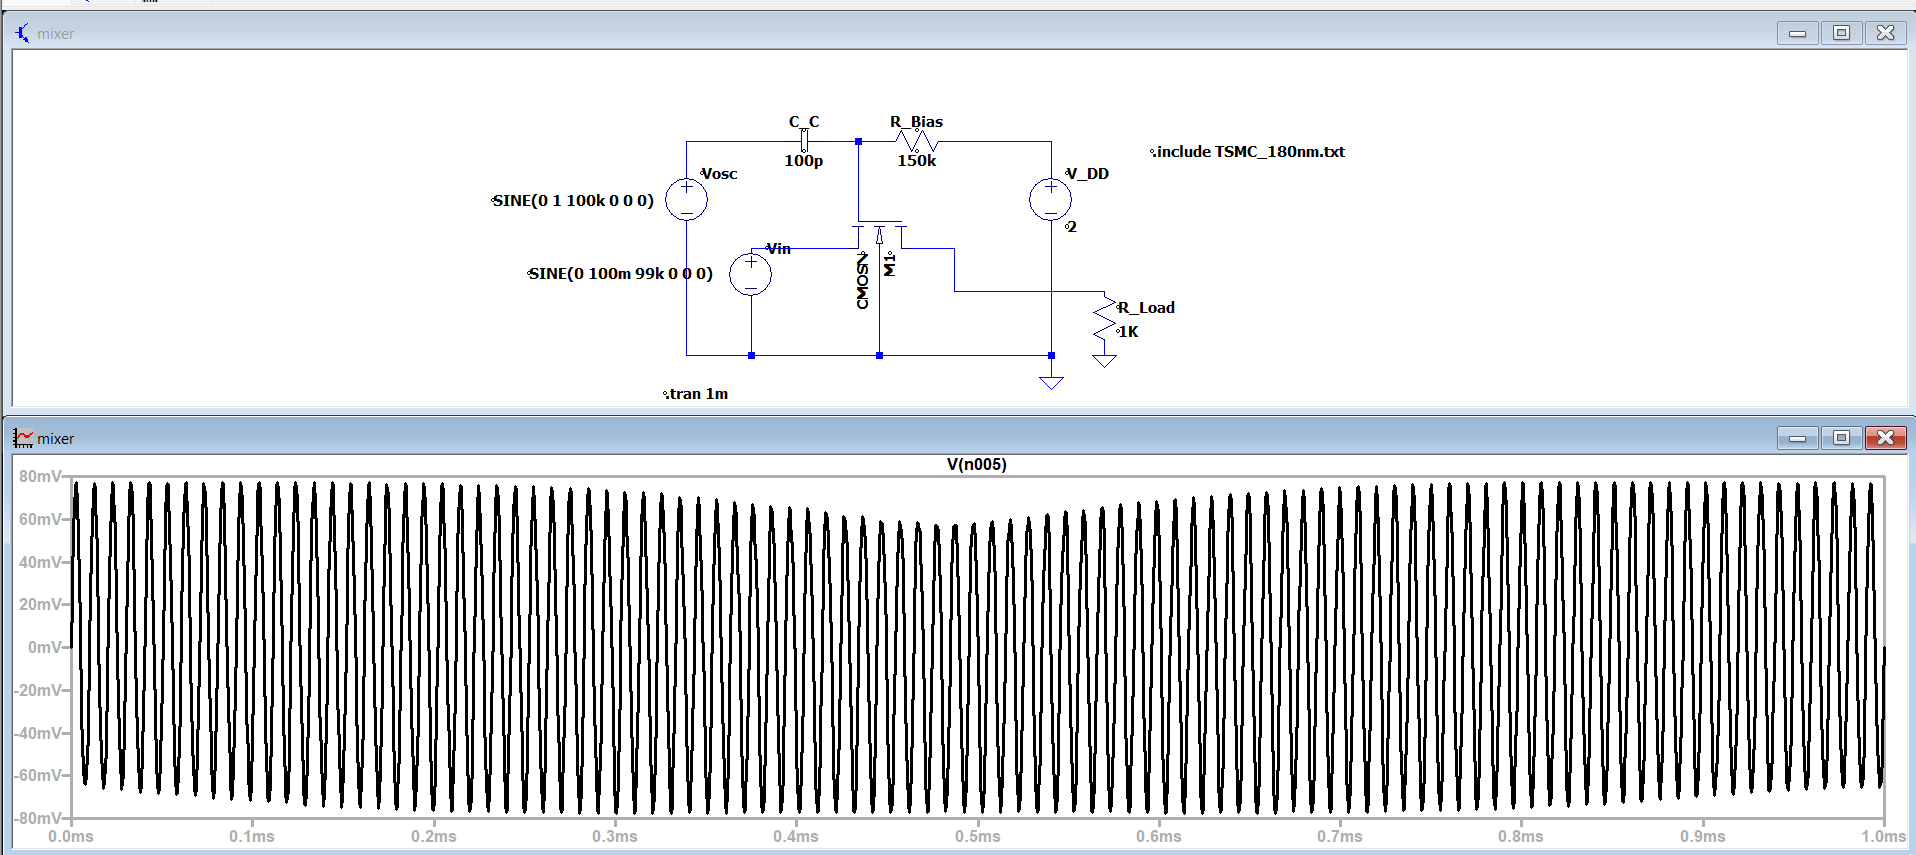
\includegraphics[width=1\linewidth]{fig/99.png}
    \caption{99kHz Output Signal}
    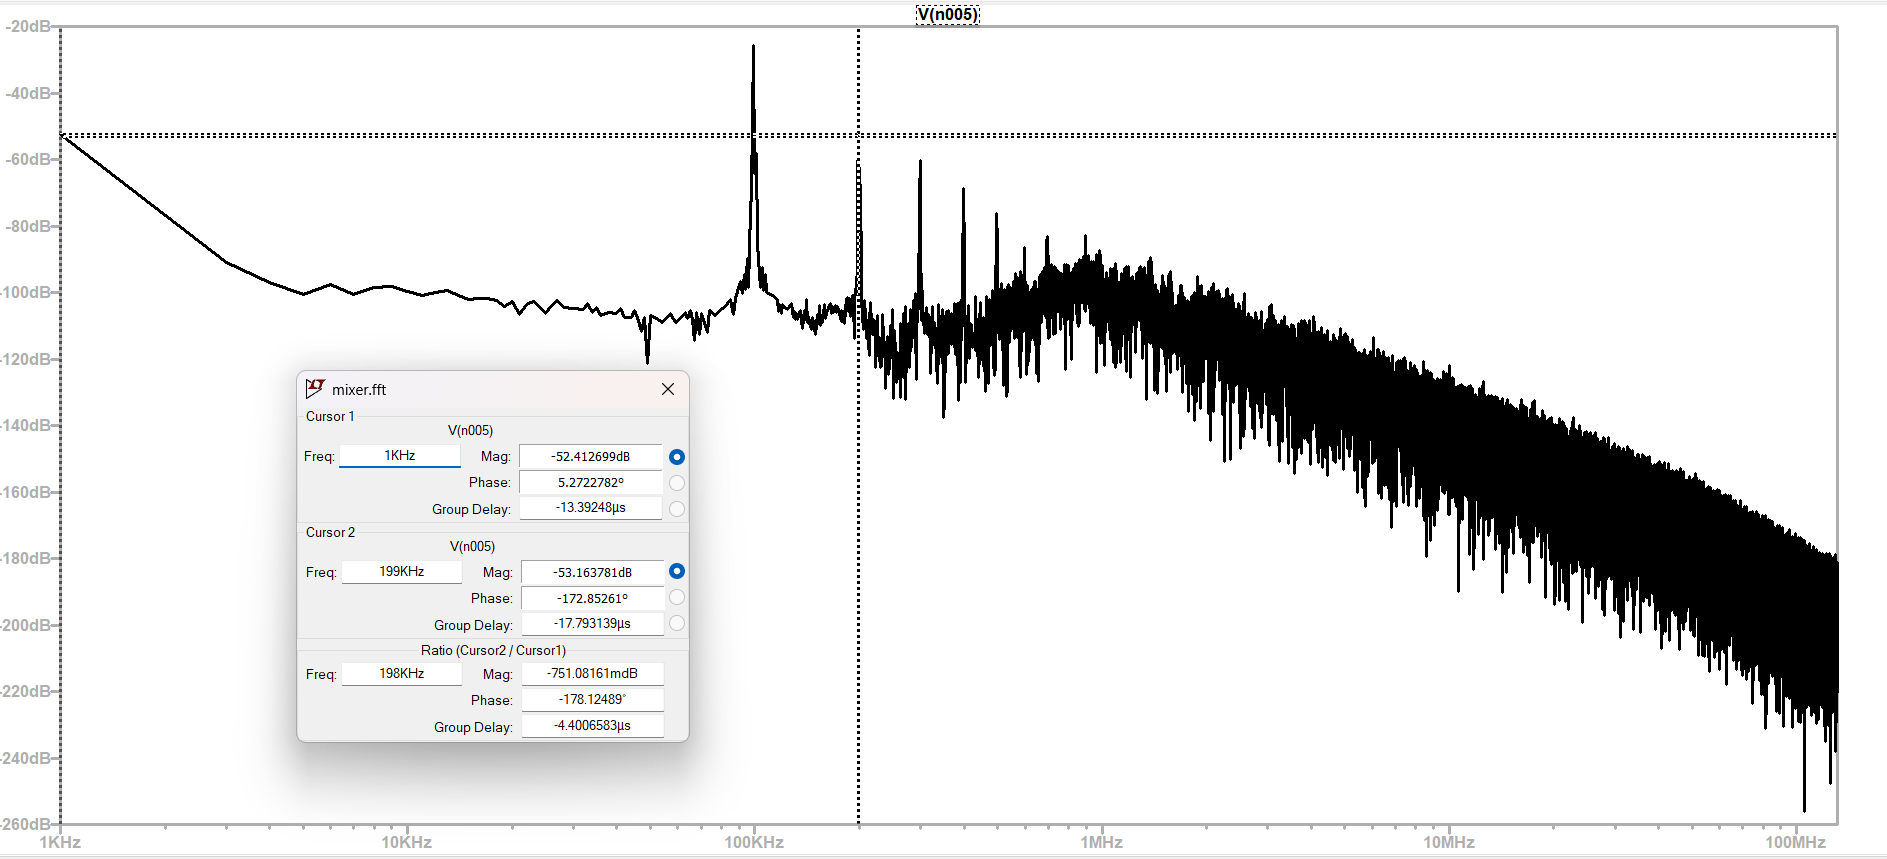
\includegraphics[width=1\linewidth]{fig/99fft.png}
    \caption{99kHz FFT}
\end{figure}
\begin{figure}
    \centering
    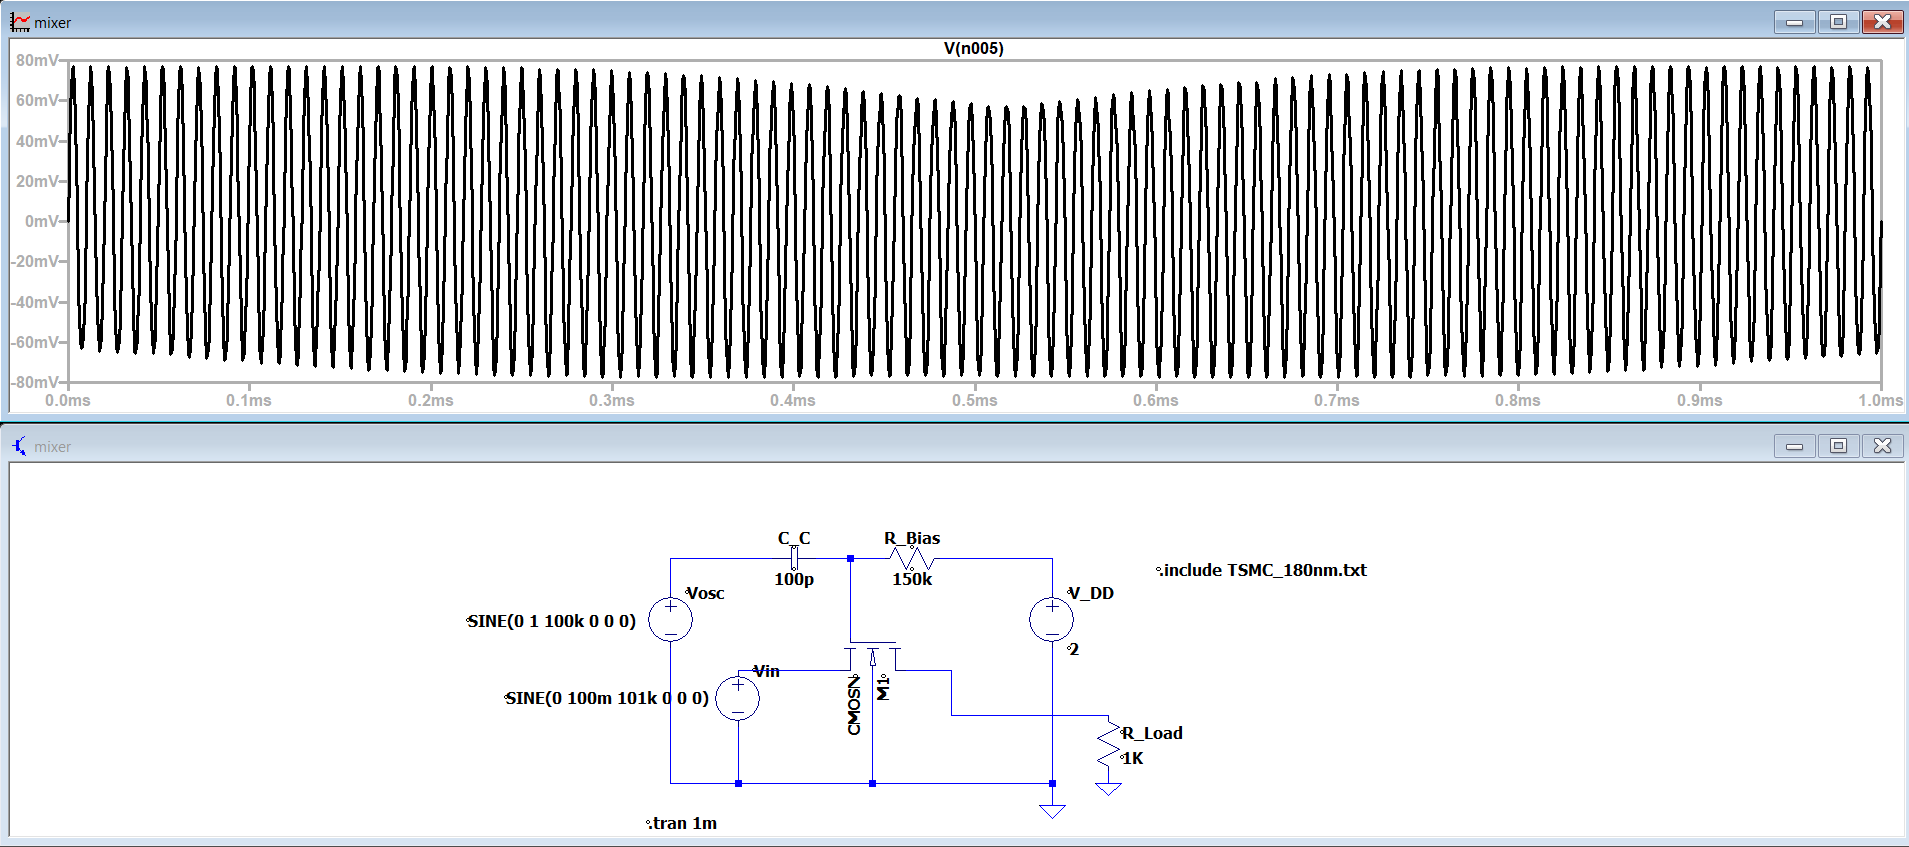
\includegraphics[width=1\linewidth]{fig/101.png}
    \caption{101kHz Output Signal}
    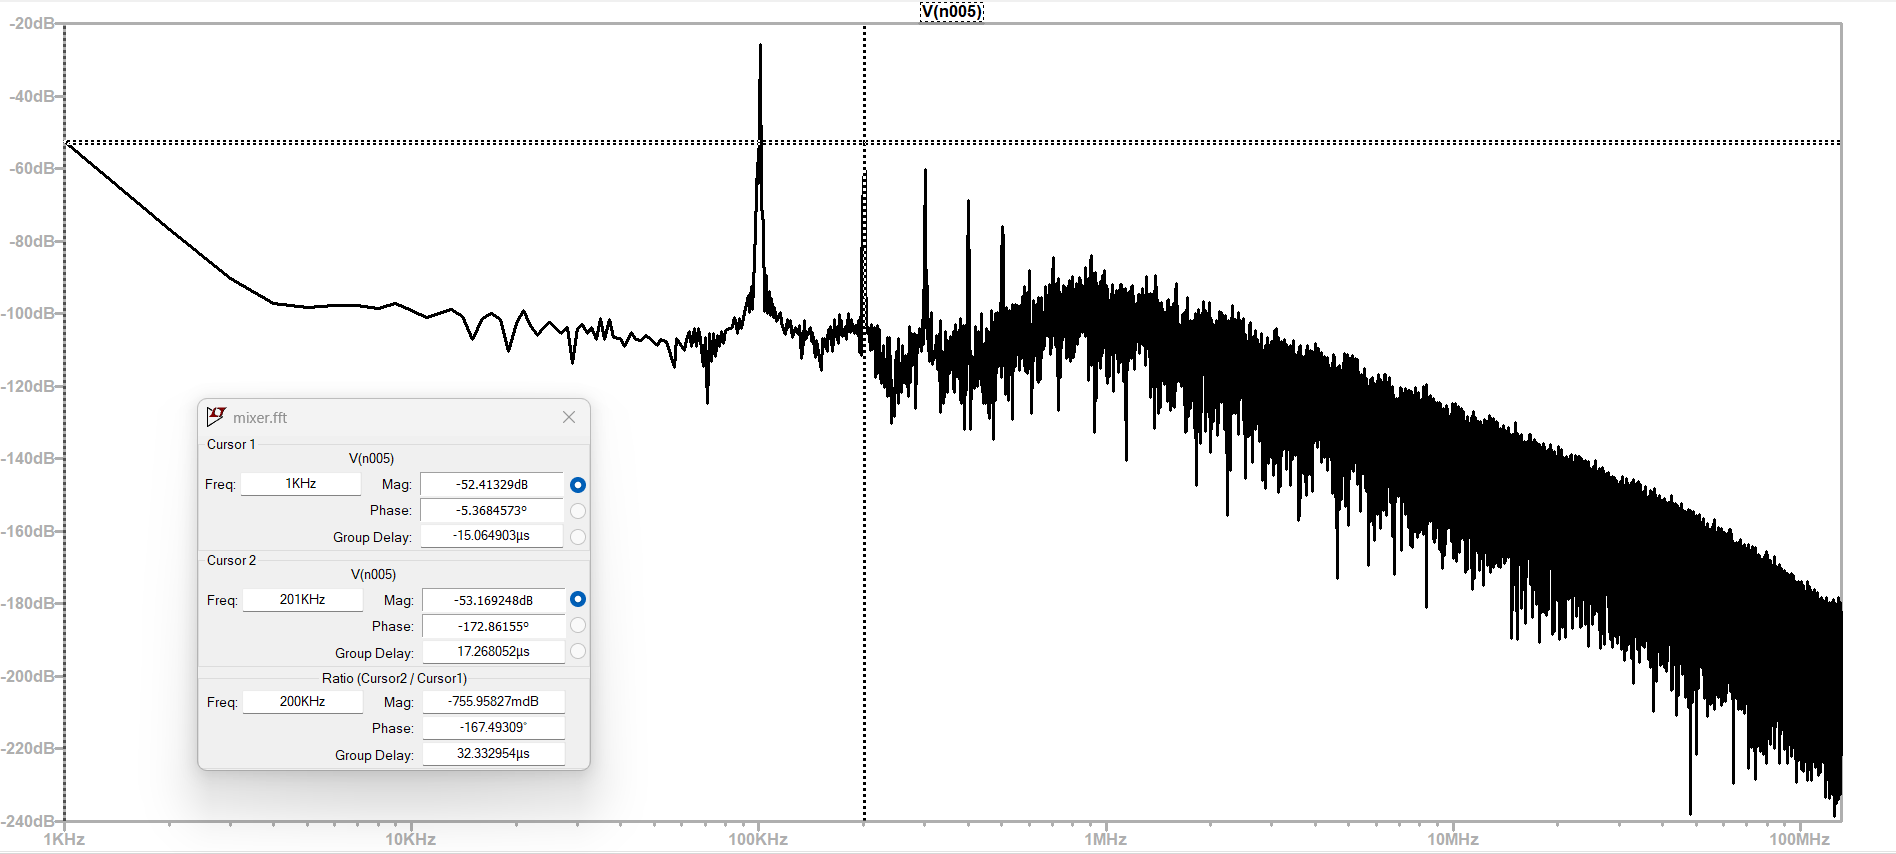
\includegraphics[width=1\linewidth]{fig/101fft.png}
    \caption{101kHz FFT}
\end{figure}
\begin{figure}
    \centering
    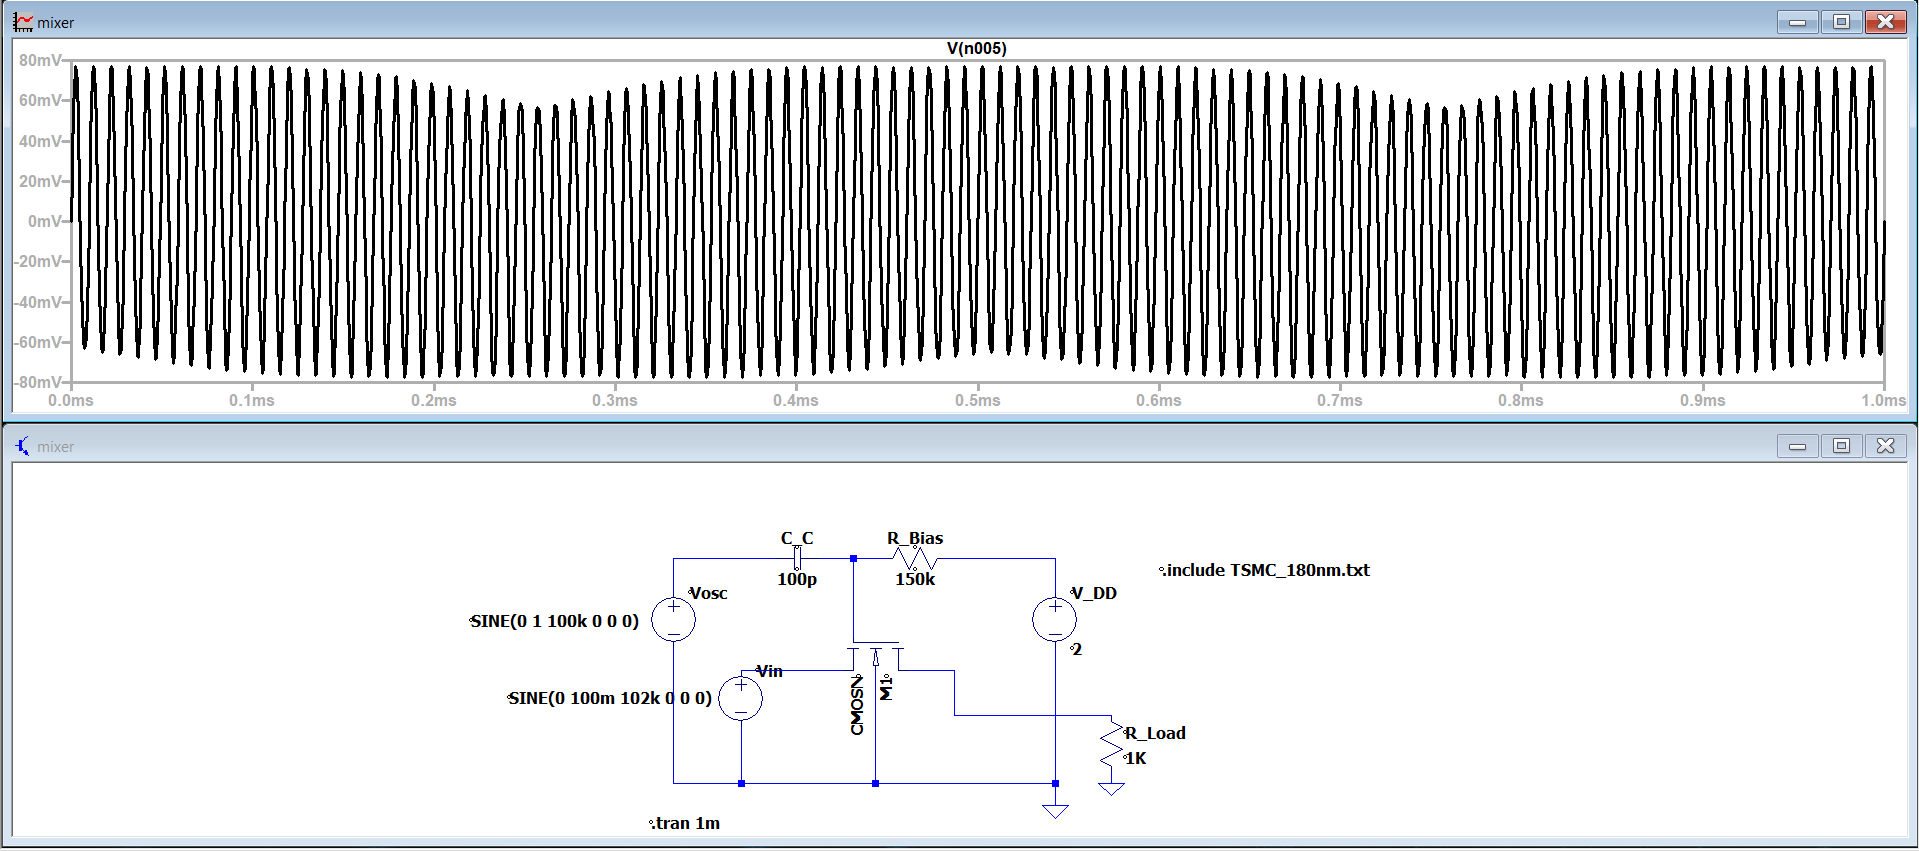
\includegraphics[width=1\linewidth]{102.png}
    \caption{102kHz Output Signal}
    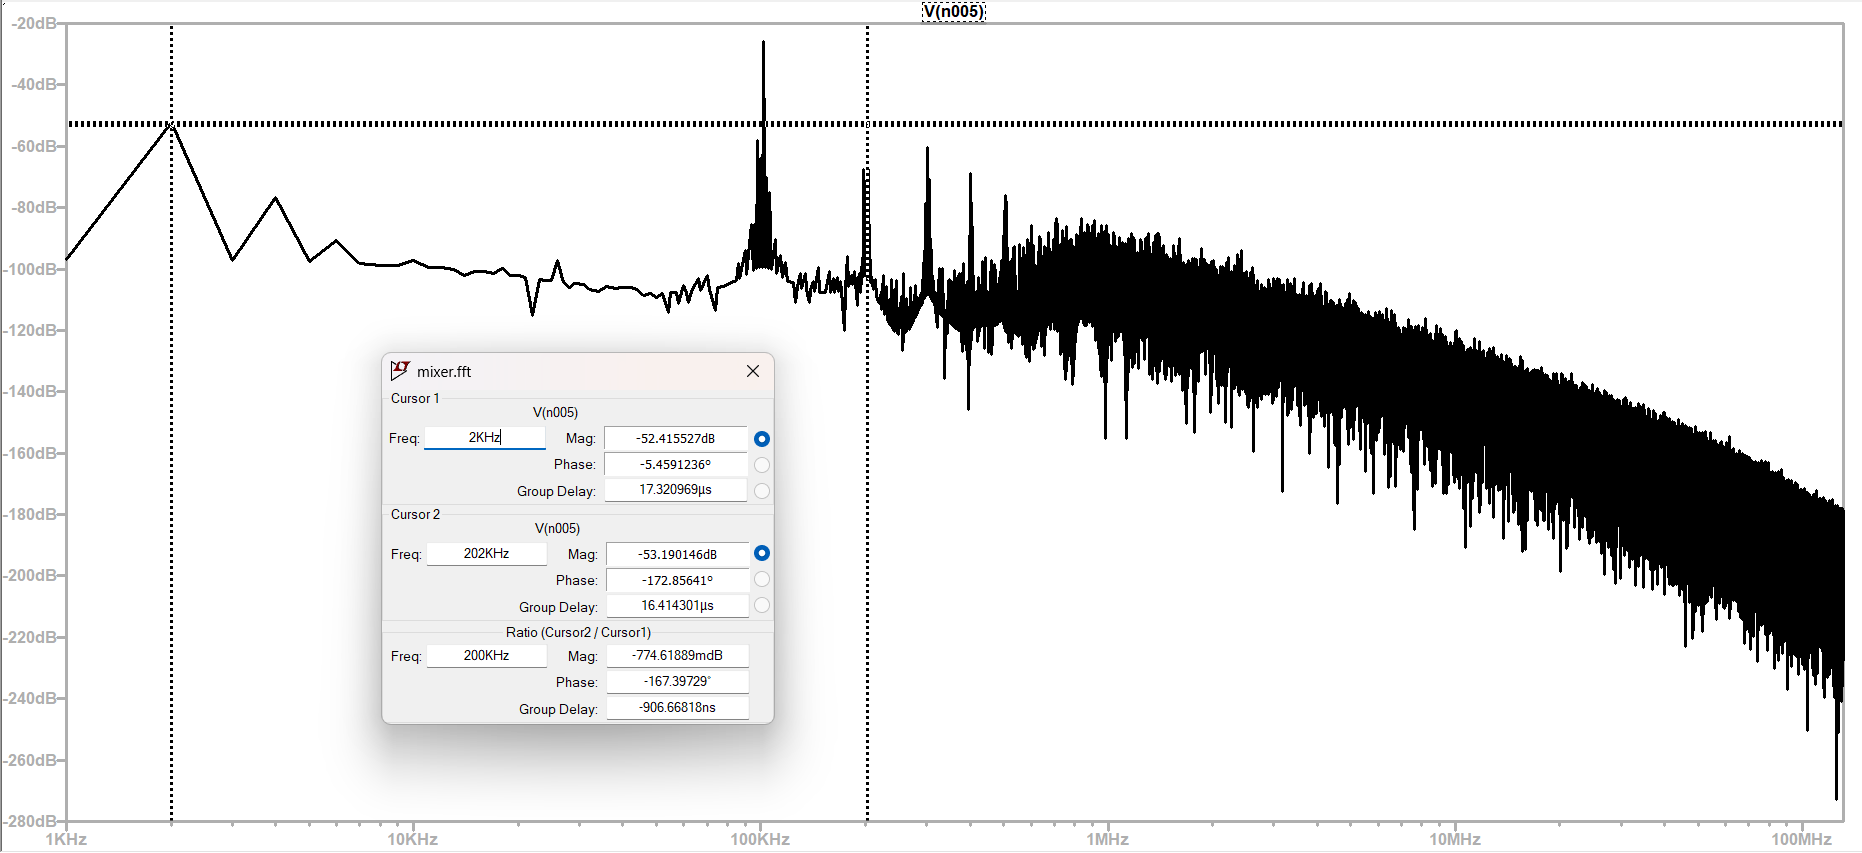
\includegraphics[width=1\linewidth]{fig/102fft.png}
    \caption{102kHz FFT}
\end{figure}
Our observations from these simulations reveal:

\begin{itemize}
    \item For $f_{in} < f_{osc}$ (when $\Delta f$ is negative): The IF signal has reversed phase compared to input.
    \item For $f_{in} > f_{osc}$ (when $\Delta f$ is positive): The IF signal maintains same phase relationship.
    \item In all cases, the difference frequency $|\Delta f| = |f_{in} - f_{osc}|$ clearly appears in the output.
    \item The FFT analysis confirms the presence of all expected frequency components:
        \begin{itemize}
            \item Difference frequency ($|\Delta f|$)
            \item Sum frequency ($f_{in} + f_{osc}$ or $2f_{osc} + \Delta f$)
            \item Input frequency leakage ($f_{in}$ or $f_{osc} + \Delta f$)
            \item LO leakage ($f_{osc}$)
        \end{itemize}
\end{itemize}
\subsection{Analysis of Phase Relationships and Image Frequency Problem}

An important observation from our mixer simulations with different input frequencies is the behavior when using input signals equidistant from the LO frequency. As shown in Fig.~\ref{fig:nmos_mixer}, we tested the mixer with both $f_{in} = 105$ kHz ($\Delta f = +5$ kHz) and $f_{in} = 95$ kHz ($\Delta f = -5$ kHz). Despite having different input frequencies, both produced remarkably similar output waveforms.

\begin{figure}[H]
    \centering
    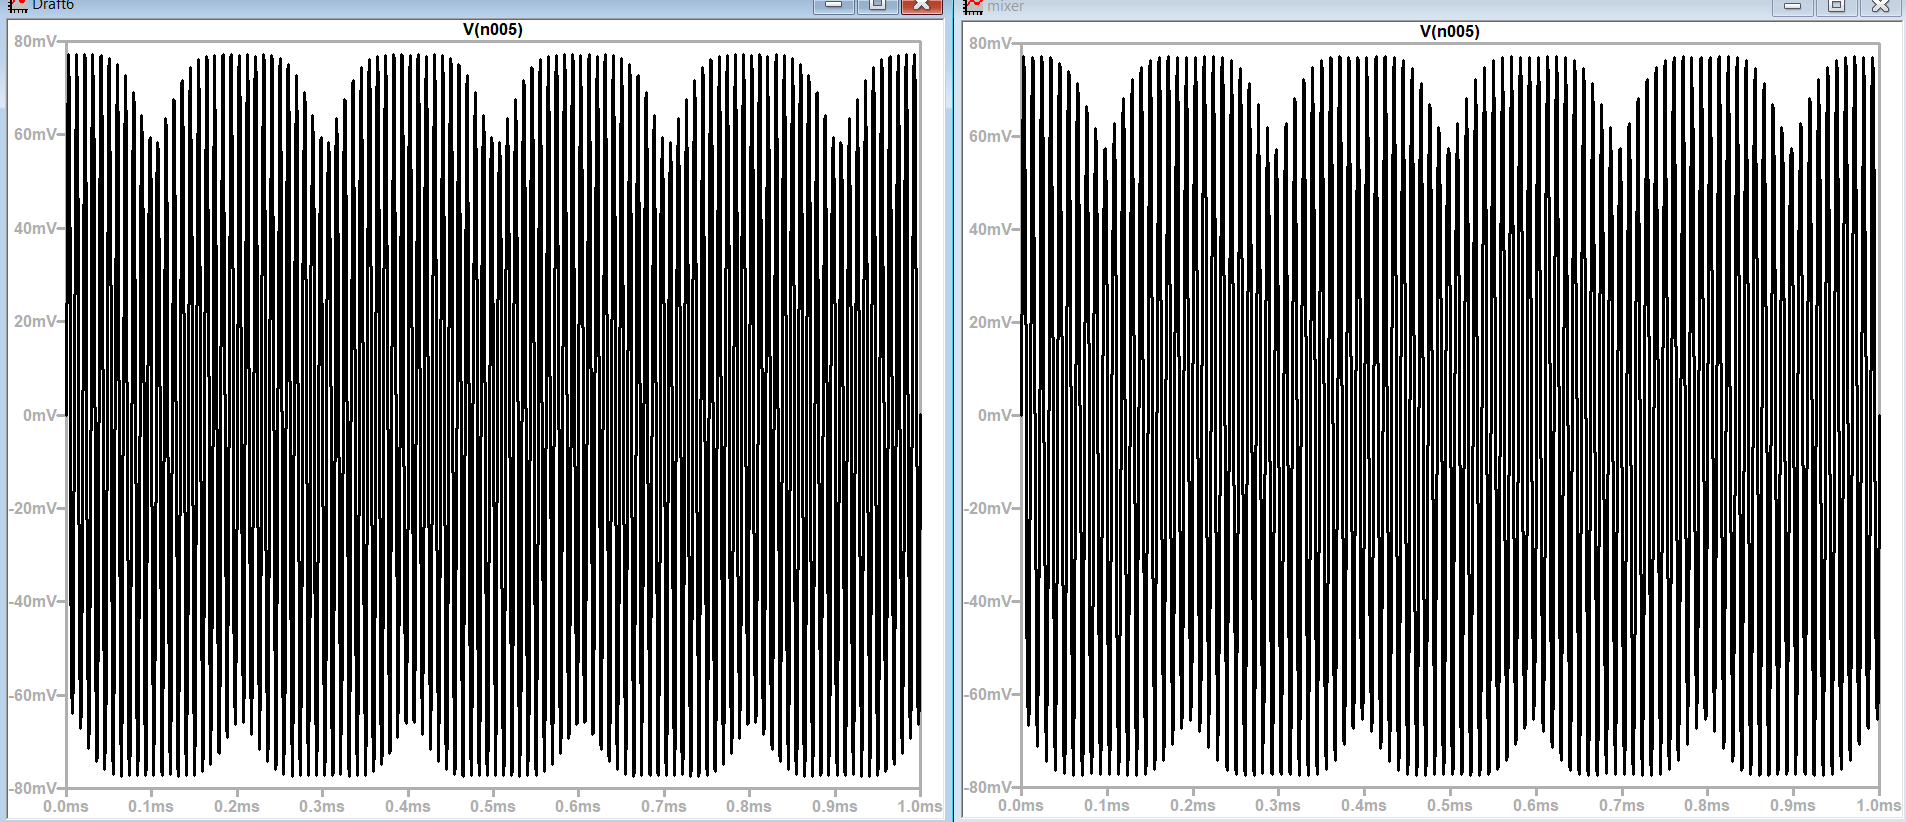
\includegraphics[width=1\linewidth]{fig/compare.png}
    \caption{Comparison of Mixer Outputs for $f_{in} = 105$ kHz and $f_{in} = 95$ kHz}
    \label{fig:image_frequency}
\end{figure}

This similarity occurs because:

\begin{itemize}
    \item Both produce the same absolute intermediate frequency: $|f_{in} - f_{osc}| = 5$ kHz in both cases
    \item Both display identical beat patterns with an envelope frequency of 5 kHz
    \item Both have similar amplitude ranges (approximately $-80$ mV to $+80$ mV)
\end{itemize}

The key difference between these two cases is theoretical rather than visual. When $f_{in} > f_{osc}$ (105 kHz case), the IF signal maintains the same phase relationship as the input, while when $f_{in} < f_{osc}$ (95 kHz case), the IF signal should exhibit a reversed phase.

Mathematically, this phase inversion occurs because when $\Delta f$ is negative, the term $\cos((\omega_{in} - \omega_{osc})t)$ becomes $\cos((\omega_{osc} - \omega_{in})t) = \cos(-(\omega_{in} - \omega_{osc})t) = \cos((\omega_{in} - \omega_{osc})t + \pi)$, introducing a 180° phase shift.

This similarity demonstrates the classic "image frequency" problem in single mixer systems, where two different input frequencies ($f_{osc} \pm \Delta f$) produce nearly identical outputs. This ambiguity between positive and negative frequency offsets highlights the importance of quadrature down-conversion in modern wireless receivers, where the phase relationships between I and Q channels enable discrimination between signals above and below the LO frequency.

These simulation results confirm that our NMOS mixer successfully performs the frequency translation function required for the quadrature down converter, with the output containing the desired intermediate frequency components that can be further processed by the subsequent low-pass filter stage.


\section{The Low Pass Filter}
\label{sec:low_pass_filter}
\subsection{Design of Second-Order Low-Pass Filter}

A second-order low-pass filter attenuates frequencies above the cutoff frequency more sharply than a first-order filter, typically providing a slope of $-40$ dB/decade. These filters are commonly used in signal processing to allow low-frequency signals to pass while reducing high-frequency noise or interference.

In this design, we use the Sallen-Key topology which is widely implemented due to its simplicity and effectiveness using op-amps. The standard Sallen-Key configuration is shown below:

\begin{figure}[H]
    \centering
    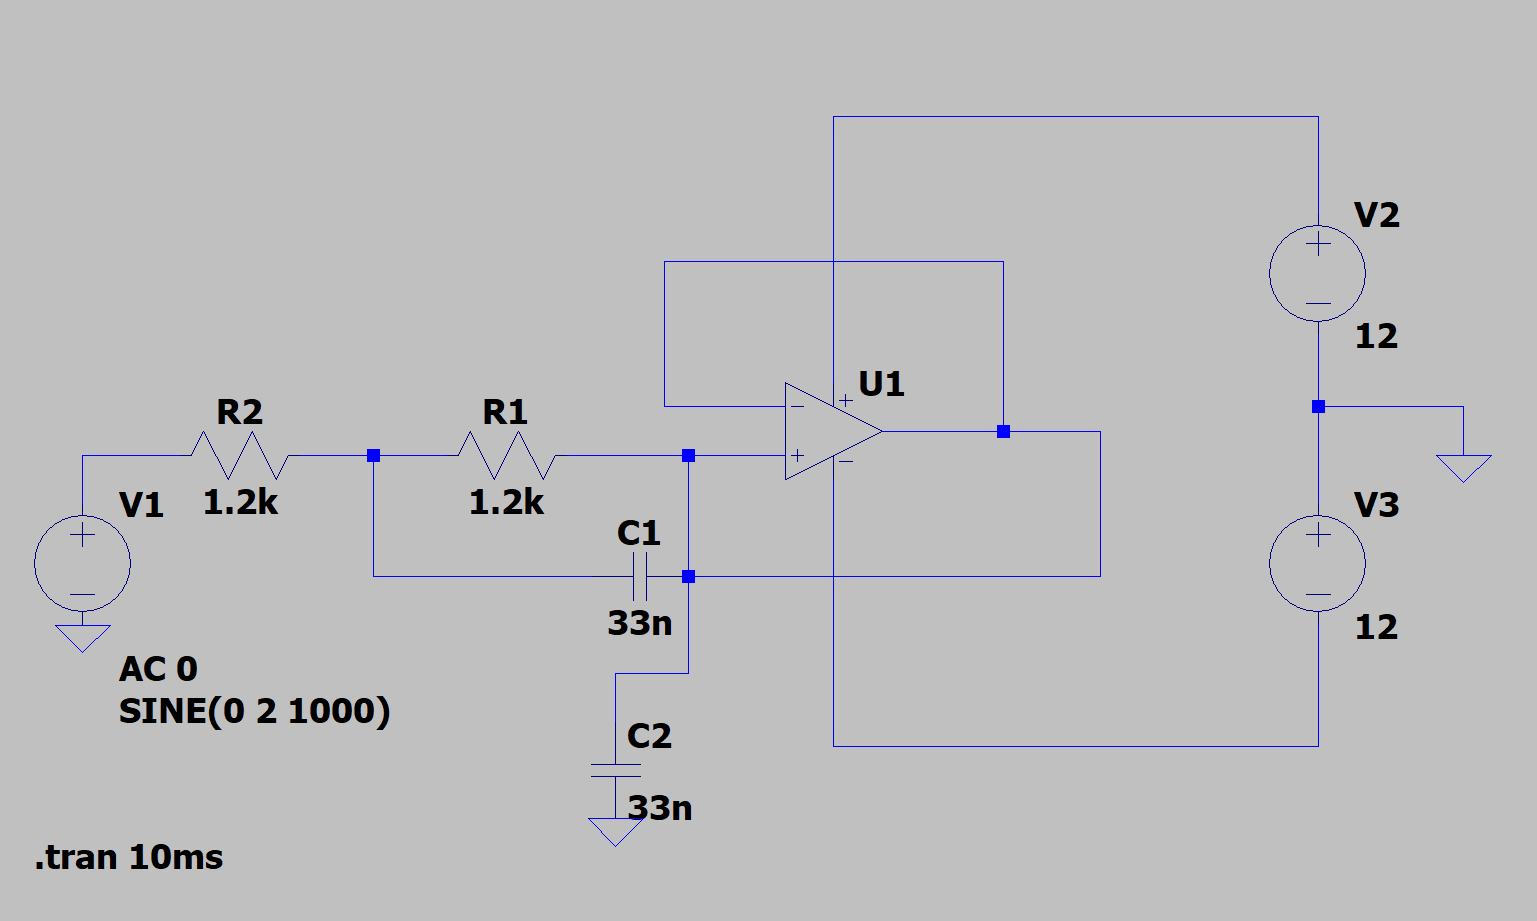
\includegraphics[width=0.9\linewidth]{sec/low-pass/helloworld.png}
    \caption{Sallen-Key Second-Order Low-Pass Filter}
    \label{fig:sallen-key}
\end{figure}

\begin{figure}[H]
    \centering
    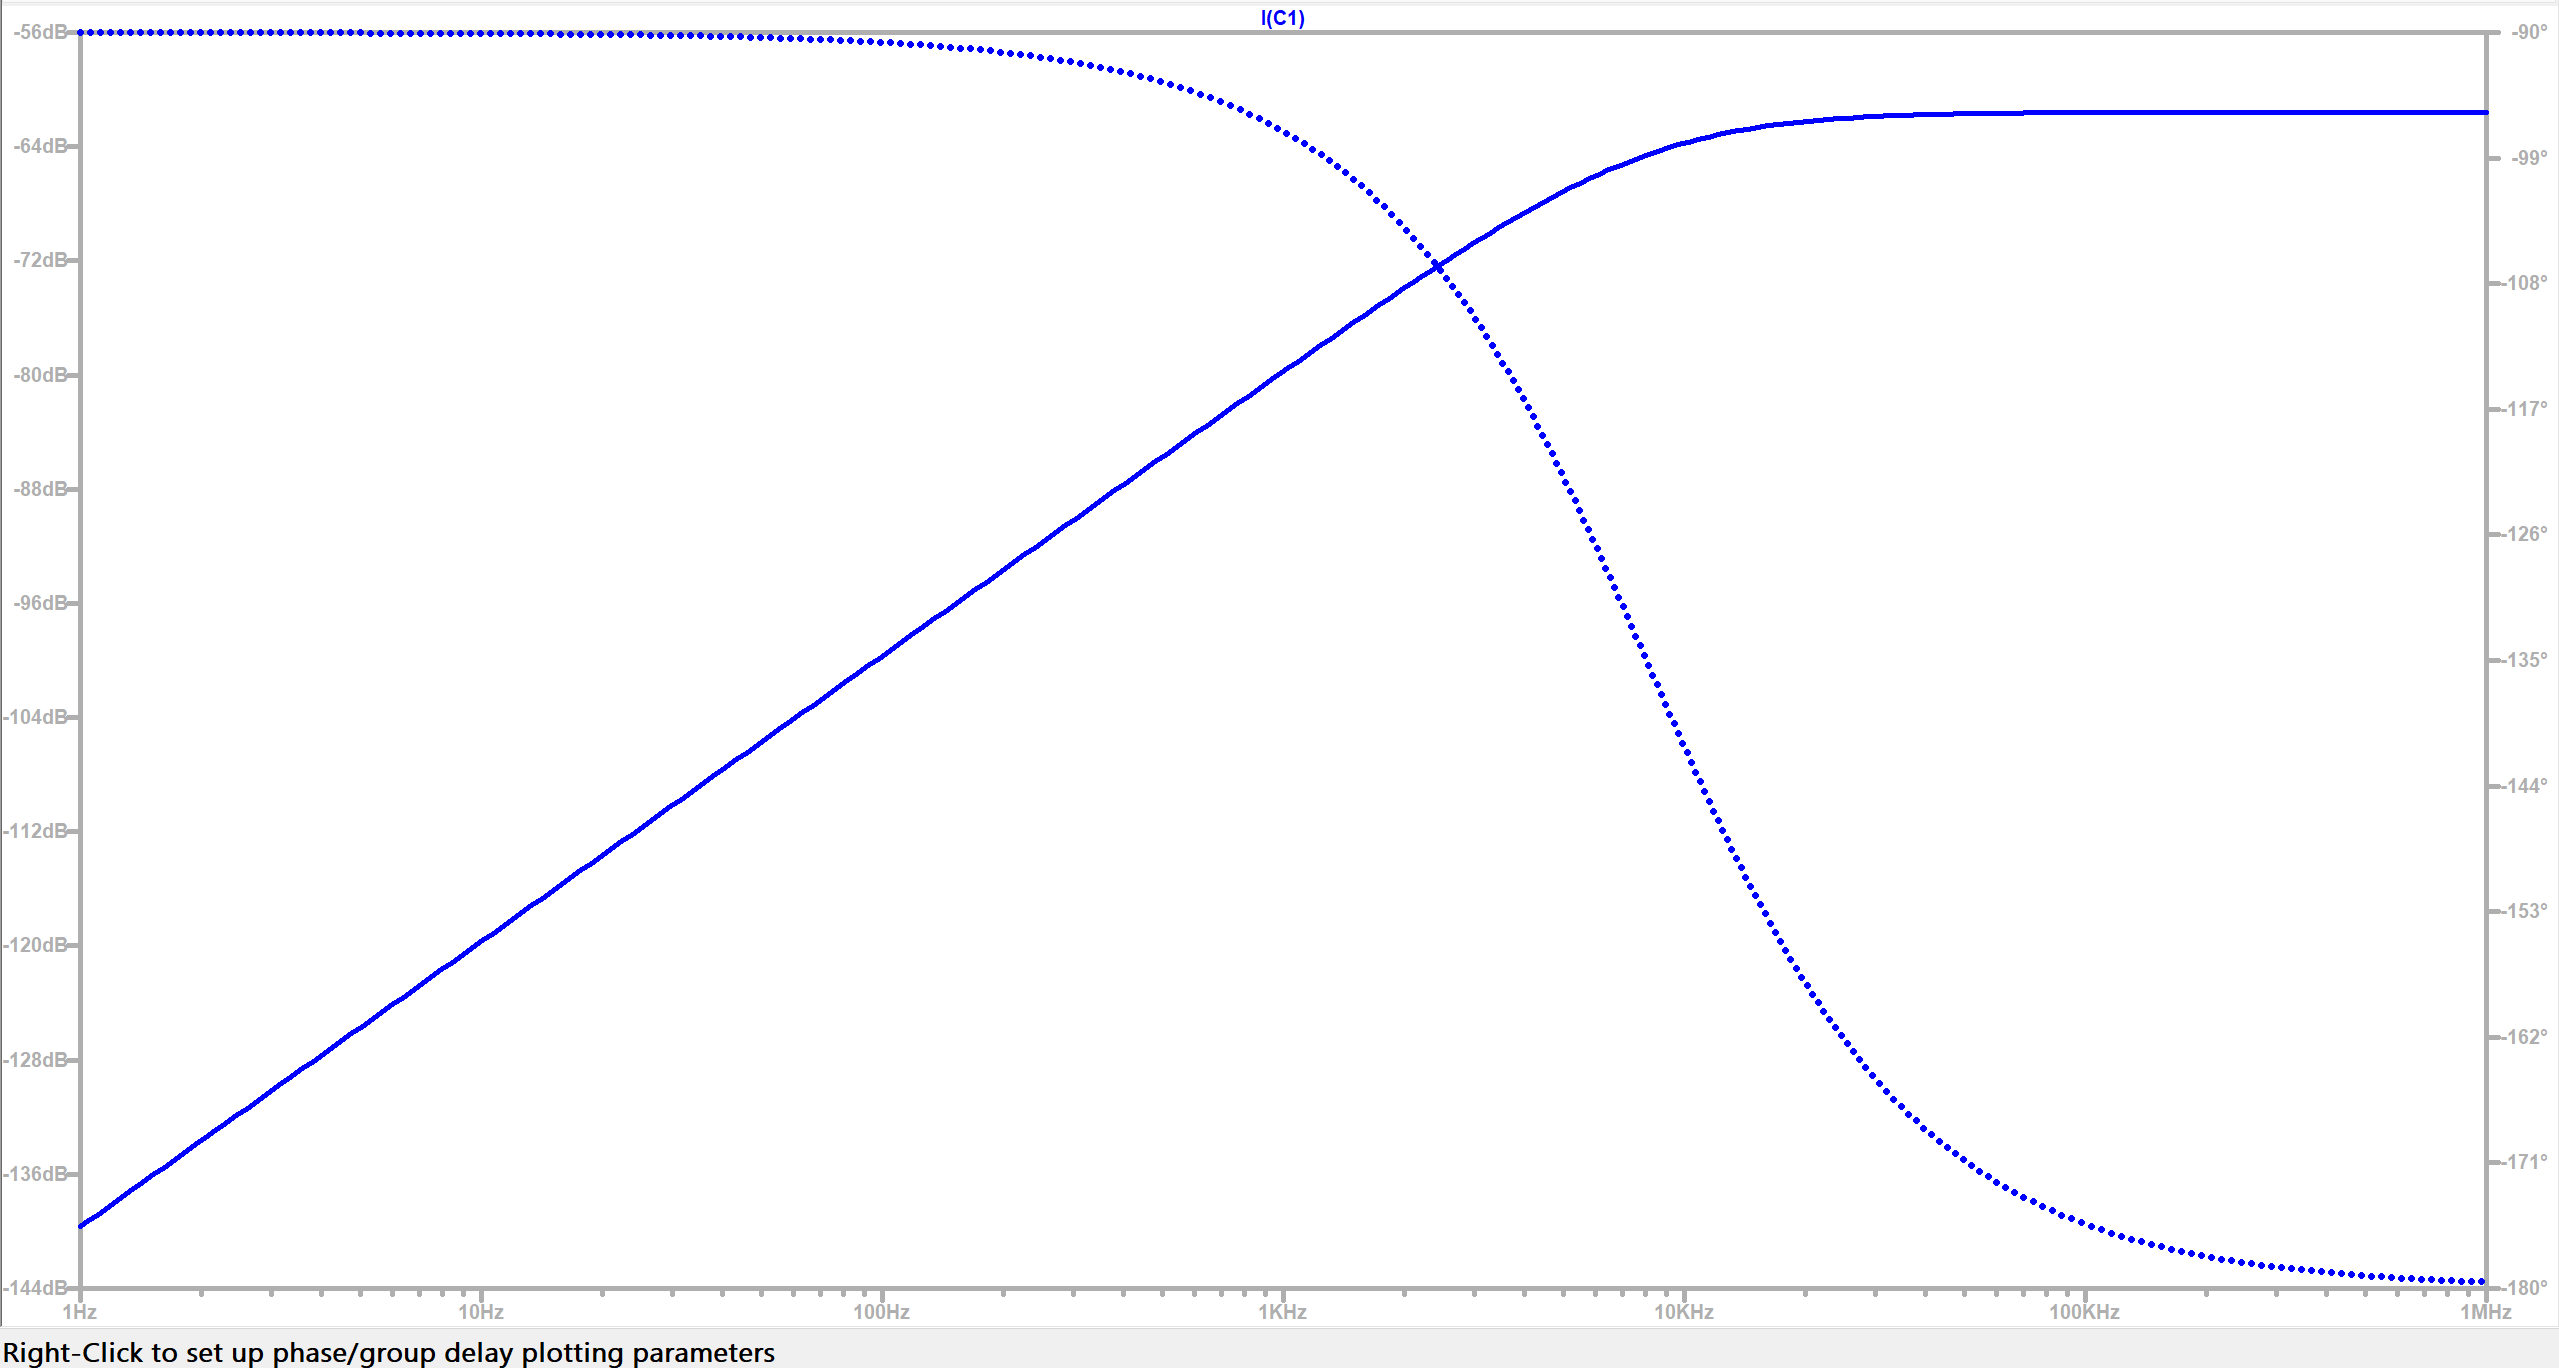
\includegraphics[width=0.95\linewidth]{sec/low-pass/image.png}
    \caption{Bode Plot of Low Pass Filter}
    \label{fig:enter-label}
\end{figure}

The transfer function of a Sallen-Key low-pass filter is given by:

\[
H(s) = \frac{1}{s^2 R_1 R_2 C_1 C_2 + s(R_1 C_1 + R_1 C_2 + R_2 C_2) + 1}
\]

Assuming $R_1 = R_2 = R$ and $C_1 = C_2 = C$ for simplicity, the transfer function becomes:

\[
H(s) = \frac{1}{s^2 R^2 C^2 + 3sRC + 1}
\]

The cutoff frequency $f_c$ of the filter is given by:

\[
f_c = \frac{1}{2\pi RC}
\]

We are designing a low-pass filter with a cutoff frequency of $f_c = 100~\text{kHz}$. Choosing $C = 1~\text{nF}$, we can compute $R$ as:

\[
R = \frac{1}{2\pi f_c C} = \frac{1}{2\pi \cdot 10^5 \cdot 10^{-9}} \approx 1.59~\text{k}\Omega
\]

Selecting a standard resistor value, we choose $R = 1.6~\text{k}\Omega$.

\subsubsection*{Simulation and Response}

When this circuit was simulated using the values:
\[
R_1 = R_2 = 1.6~\text{k}\Omega, \quad C_1 = C_2 = 100~\text{nF}
\]

the output showed a sharp cutoff near $1000~\text{kHz}$ as expected. The gain at low frequencies remained nearly constant (unity gain), and the attenuation slope beyond the cutoff was approximately $-40$ dB/decade, confirming the second-order behavior.

\begin{figure}[H]
    \centering
    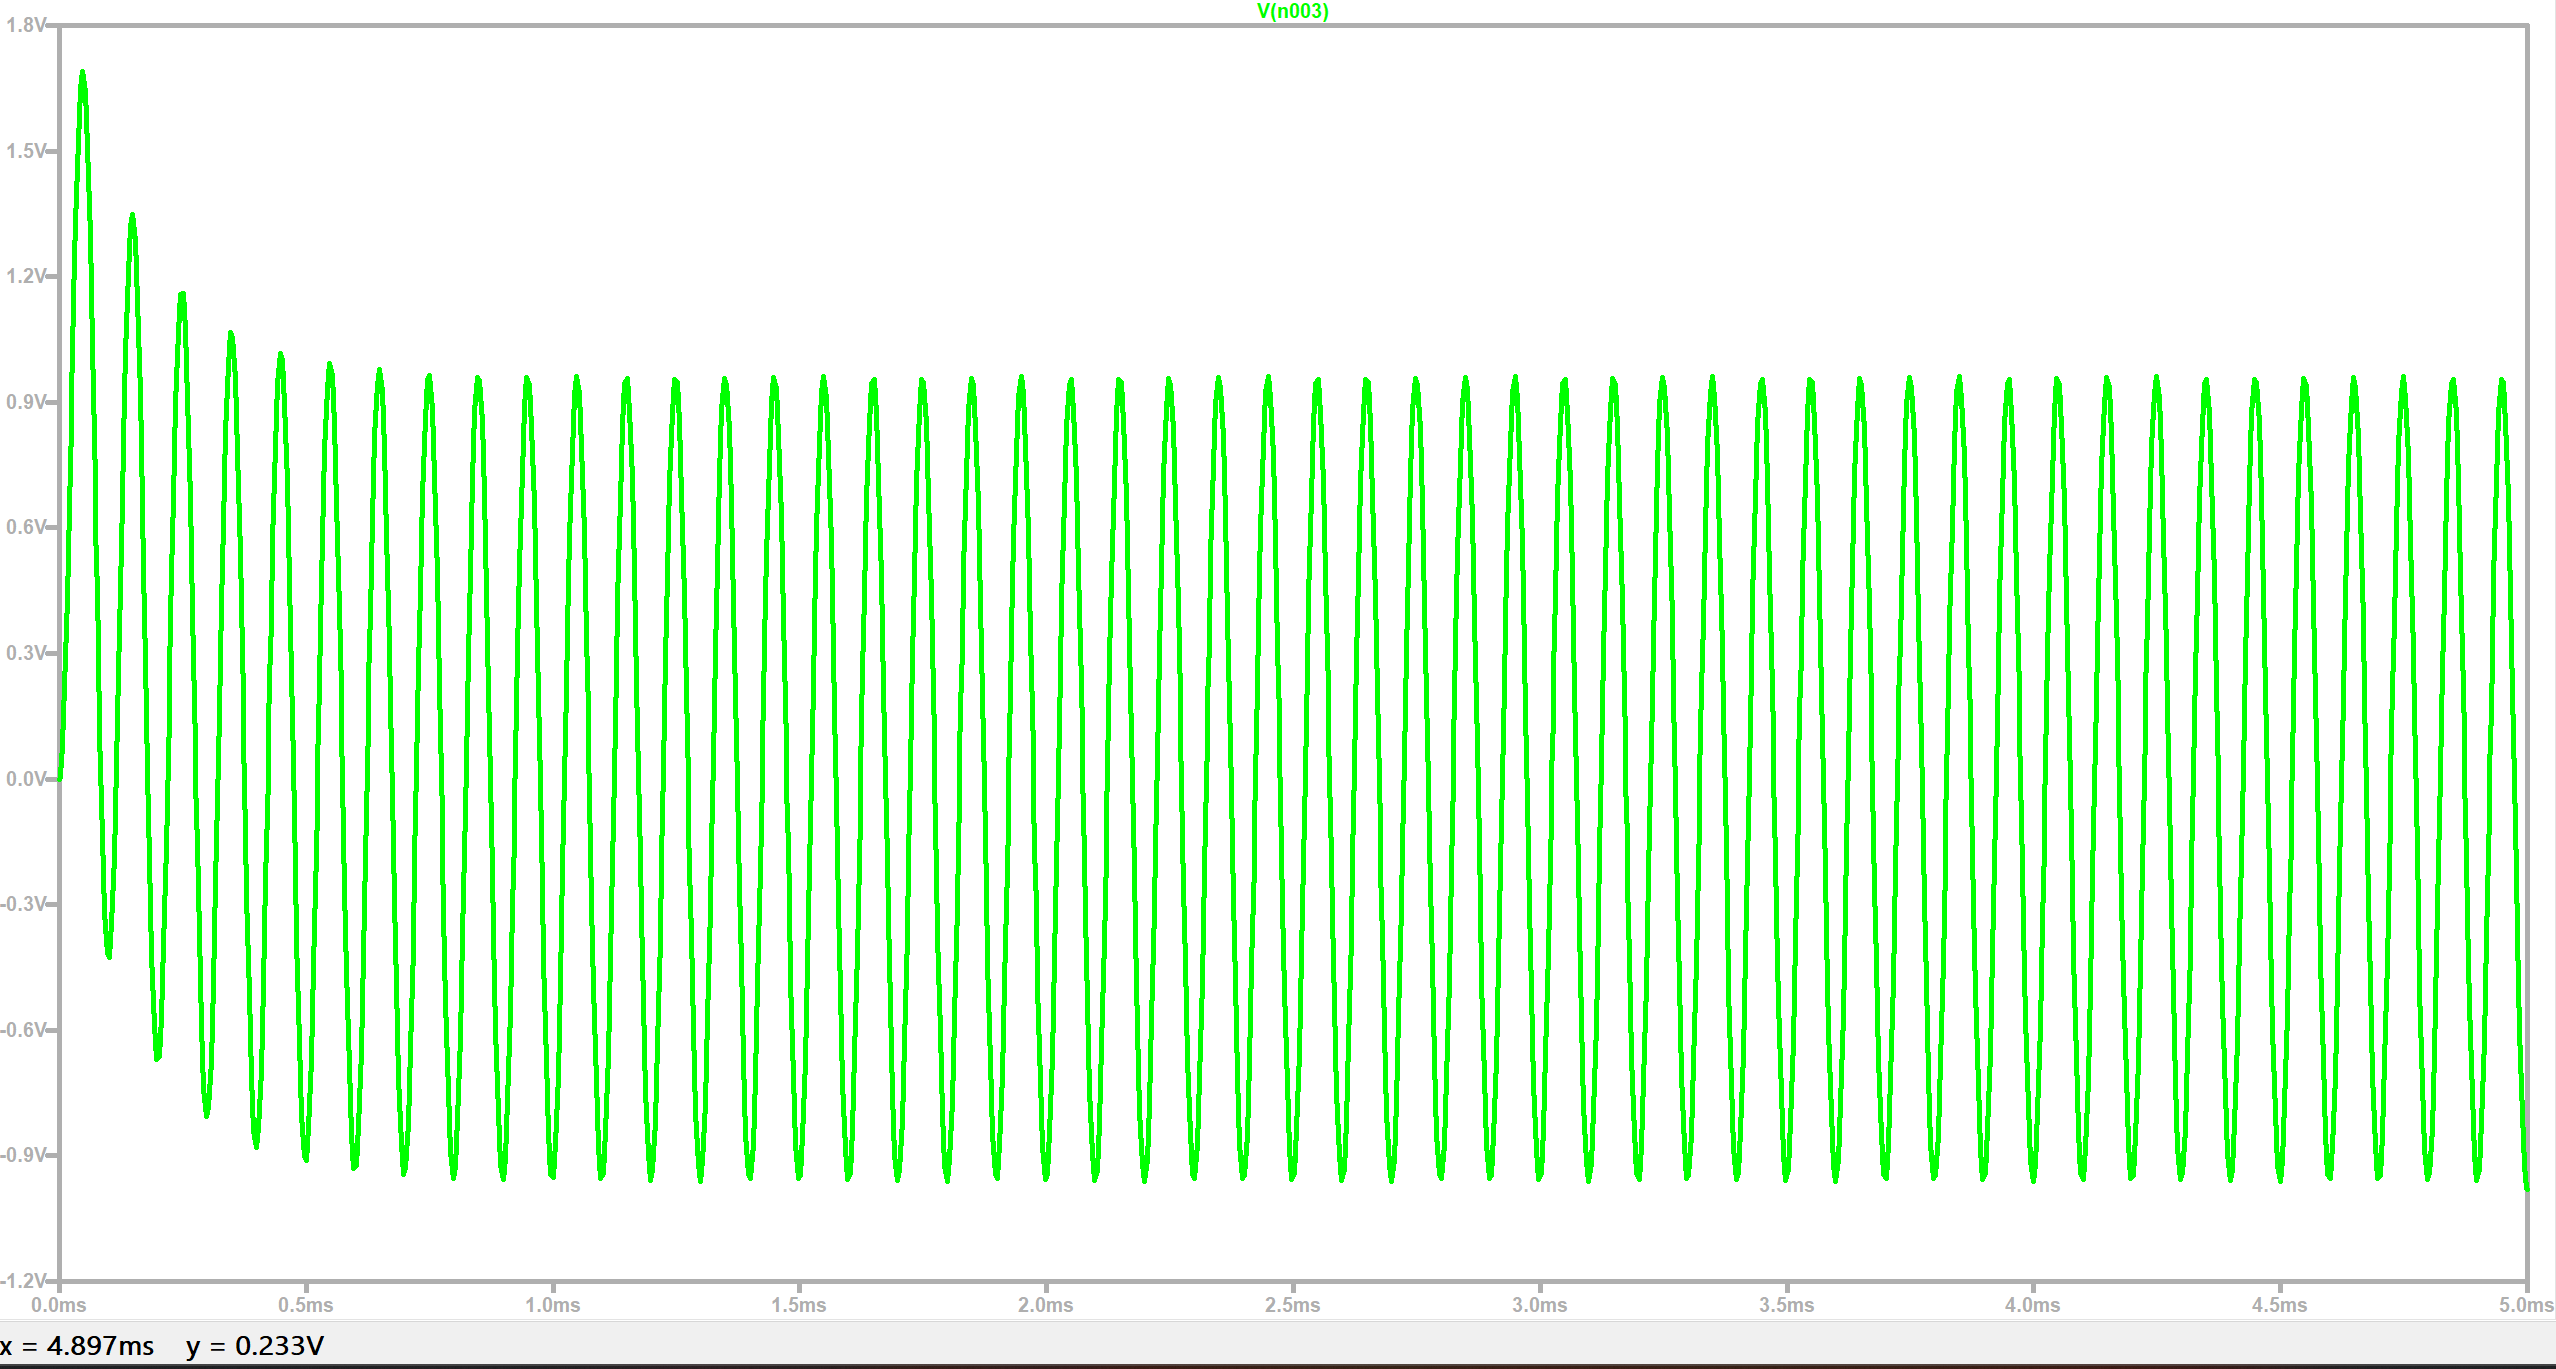
\includegraphics[width=1\linewidth]{sec/low-pass/asd.png}
    \caption{Frequency response of the Second-Order Low-Pass Filter}
    \label{fig:low-pass-response}
\end{figure}

This low-pass filter can be used in signal conditioning, especially to remove high-frequency noise from the oscillator or as a component in larger analog signal processing systems.


\subsection*{Importance of Second-Order Low-Pass Filter in a Quadrature Down-Converter}

In a \textit{quadrature down-converter}, the incoming RF signal is mixed with two local oscillator (LO) signals that are $90^\circ$ out of phase, producing the \textbf{in-phase (I)} and \textbf{quadrature (Q)} baseband components. This mixing operation generates both sum and difference frequency components.

\begin{itemize}
    \item The desired \textbf{baseband signal} appears near 0 Hz (difference frequency: RF$-$LO).
    \item Unwanted \textbf{high-frequency components}, such as the sum frequency (RF$+$LO), also appear in the mixer output.
\end{itemize}

To isolate the baseband I/Q signals, a \textbf{low-pass filter (LPF)} is applied. Specifically, a \textbf{second-order low-pass filter} is preferred due to its sharper roll-off and better attenuation of out-of-band signals compared to first-order filters.

\paragraph{Key Benefits of Using a Second-Order LPF:}
\begin{enumerate}
    \item \textbf{Sharper Cutoff:} Second-order filters have a roll-off rate of $-40~\text{dB/decade}$, providing more effective suppression of high-frequency mixer products.
    
    \item \textbf{Improved Selectivity:} It better isolates the desired baseband signal by reducing adjacent channel interference.
    
    \item \textbf{Anti-Aliasing Protection:} When followed by analog-to-digital conversion (ADC), the LPF prevents aliasing by attenuating frequencies above the Nyquist limit.
    
    \item \textbf{Noise Reduction:} Suppresses out-of-band noise, improving the signal-to-noise ratio (SNR) of the baseband signal.
    
    \item \textbf{Defines Bandwidth:} The filter determines the usable signal bandwidth and thus helps shape the system's frequency response.
\end{enumerate}


\section{Combined Results}
\label{sec:result}
\subsection{Quadrature Down-Converter: Circuit Integration and Results}

A quadrature down-converter is used to shift a high-frequency input signal down to baseband using quadrature mixing. It uses two key signals from the quadrature oscillator: an in-phase (I) signal and a quadrature-phase (Q) signal, each $90^\circ$ out of phase with each other. The incoming RF signal is mixed with these two components to generate two separate down-converted signals. These are then passed through low-pass filters to isolate the baseband components.

\subsubsection{Schematic of the Quadrature Down-Converter}

\begin{figure}[H]
    \centering
    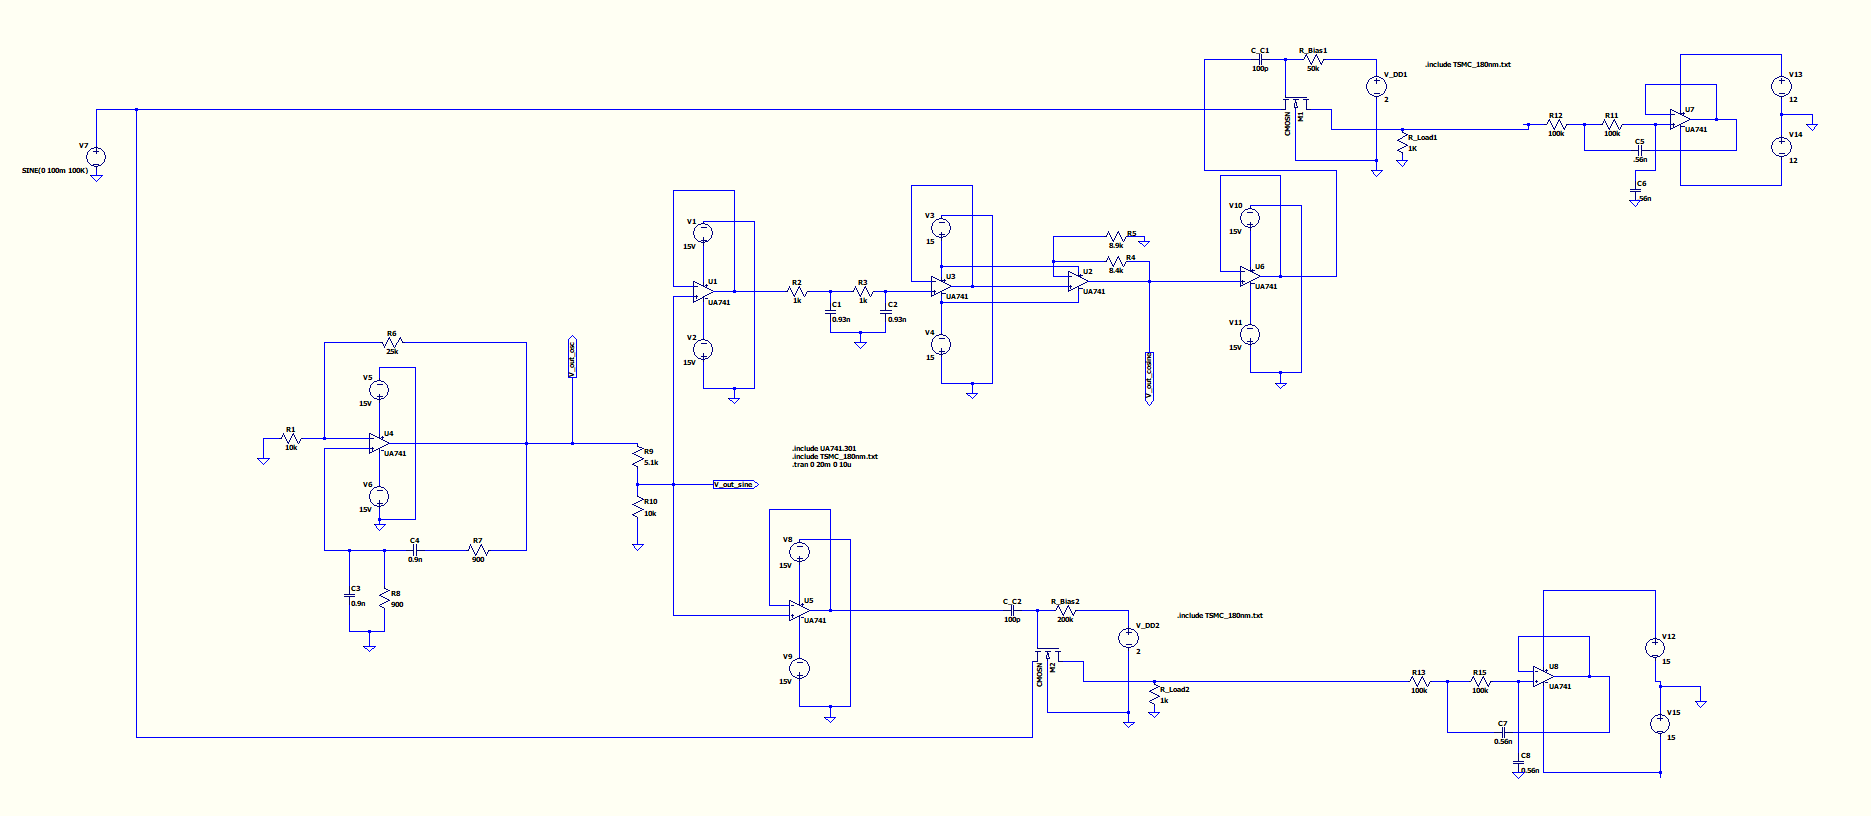
\includegraphics[width=1\linewidth]{sec/sch.png}
    \caption{Complete Quadrature Down-Converter Circuit: Mixer + Quadrature Oscillator + 2nd Order Low Pass Filter}
    \label{fig:quad-downconv-schematic}
\end{figure}
\begin{figure}[H]
    \centering
    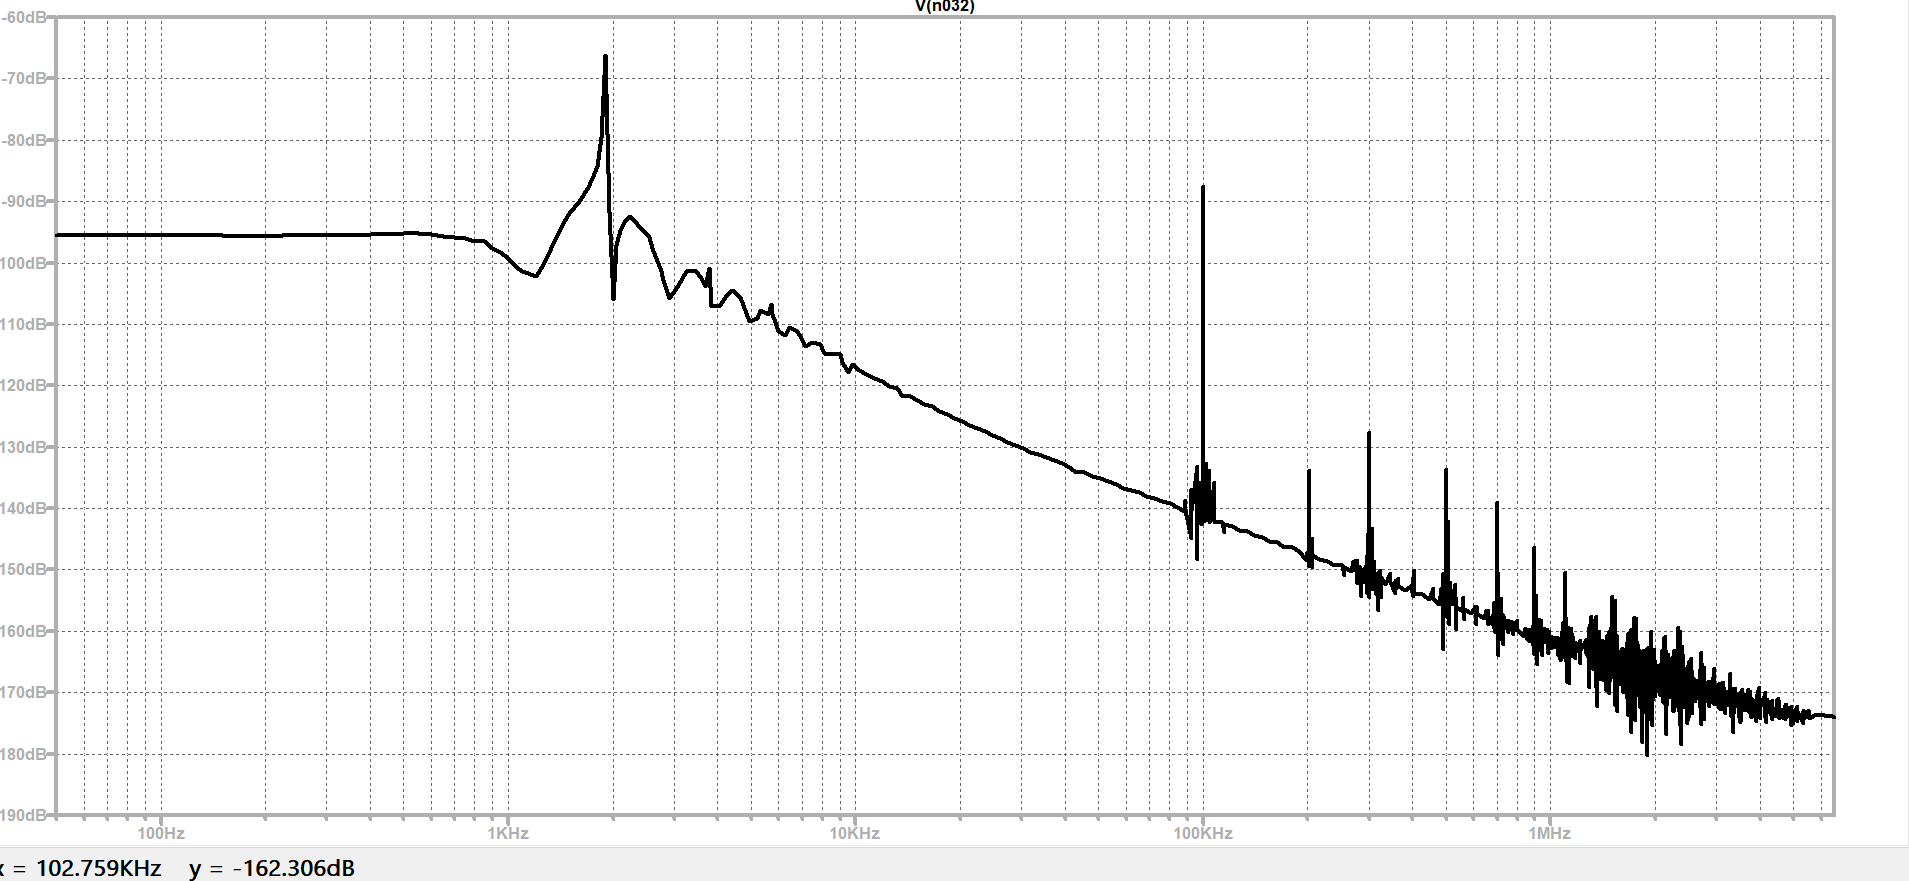
\includegraphics[width=0.95\linewidth]{sec/ffts.png}
    \caption{FFT Analysis of I and Q Outputs}
    \label{fig:fft-analysis}
\end{figure}

As shown in \Cref{fig:quad-downconv-schematic}, the circuit integrates the following components:
\begin{itemize}
    \item \textbf{Quadrature Oscillator:} Generates $100\text{ kHz}$ sinusoidal signals with $90^\circ$ phase difference.
    \item \textbf{Mixer:} Multiplies the incoming high-frequency signal (RF input) with both the I and Q oscillator signals.
    \item \textbf{2nd Order Low-Pass Filters:} Extract the baseband (low-frequency) components from the mixer outputs.
\end{itemize}

\subsubsection{Operation and Frequency Translation}

The RF input signal is defined as:
\[
V_{RF} = A \cos(2\pi f_{RF} t)
\]
where $f_{RF} = 100.1\text{ kHz}$ and $A$ is the amplitude of the RF signal.

Let the oscillator signals be:
\[
V_I = \cos(2\pi f_{LO} t), \quad V_Q = \sin(2\pi f_{LO} t)
\]
with $f_{LO} = 100\text{ kHz}$.

The mixer outputs:
\begin{align*}
V_{mix,I} &= V_{RF} \cdot V_I = A \cos(2\pi f_{RF} t) \cos(2\pi f_{LO} t) \\
          &= \frac{A}{2} \left[ \cos(2\pi (f_{RF} - f_{LO}) t) + \cos(2\pi (f_{RF} + f_{LO}) t) \right] \\
V_{mix,Q} &= V_{RF} \cdot V_Q = A \cos(2\pi f_{RF} t) \sin(2\pi f_{LO} t) \\
          &= \frac{A}{2} \left[ \sin(2\pi (f_{RF} - f_{LO}) t) + \sin(2\pi (f_{RF} + f_{LO}) t) \right]
\end{align*}

After applying the 2nd order low-pass filter (cutoff $\ll f_{LO}$), the high-frequency terms at $f_{RF} + f_{LO}$ are removed. The outputs are:
\[
V_{I,baseband} = \frac{A}{2} \cos(2\pi \Delta f t), \quad V_{Q,baseband} = \frac{A}{2} \sin(2\pi \Delta f t)
\]
where $\Delta f = f_{RF} - f_{LO} = 100.1\text{ kHz} - 100\text{ kHz} = 0.1\text{ kHz} = 100\text{ Hz}$

\subsubsection{Simulation Results and Analysis}

\begin{figure}[H]
    \centering
    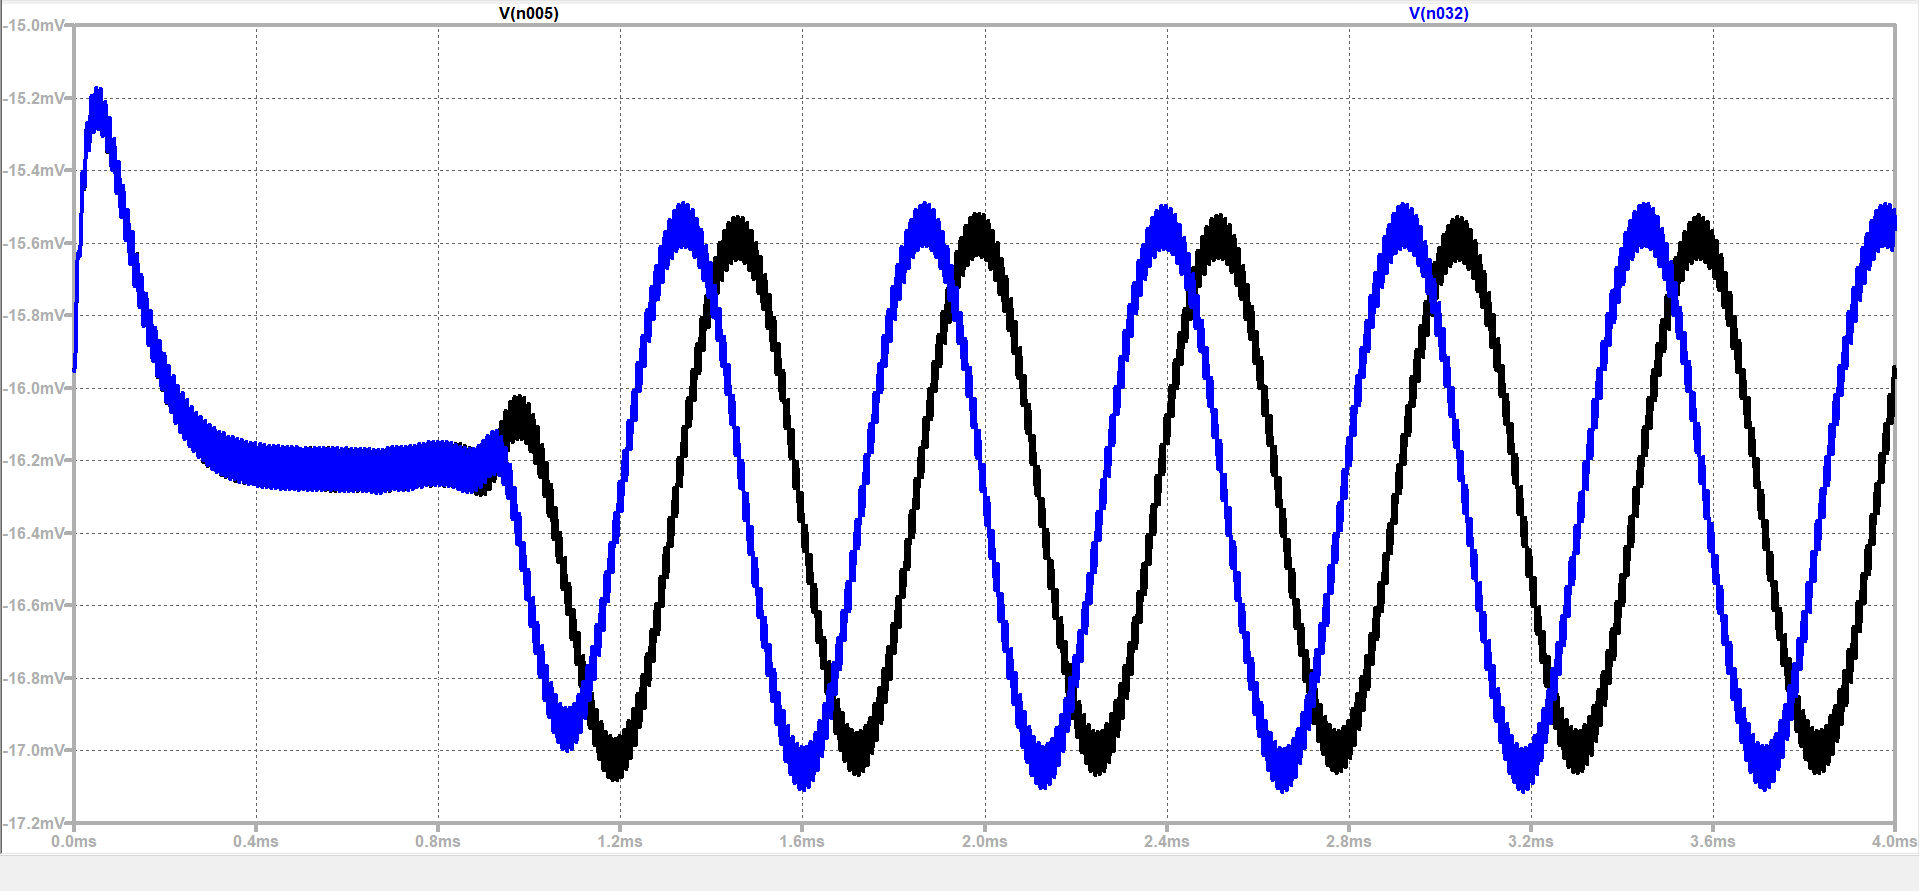
\includegraphics[width=1\linewidth]{sec/output.png}
    \caption{Simulation Output: Quadrature Down-Converted Baseband Signals (I and Q)}
    \label{fig:quad-downconv-output}
\end{figure}

Our measured results from the implemented quadrature down-converter reveal several important characteristics:

\begin{itemize}
    \item \textbf{Signal Amplitude:} The output signals are in the microvolts range, with a measured peak-to-peak amplitude of approximately $2$ mV, which is significantly lower than theoretical expectations. This low amplitude can be attributed to attenuation through the multiple stages and potential impedance mismatches in the circuit.
    
    \item \textbf{Phase Relationship:} The blue and black traces (I and Q outputs) maintain a clear $90^\circ$ phase shift, which is essential for proper quadrature operation. This phase relationship is precisely what allows the system to discriminate between signals above and below the LO frequency.
    
    \item \textbf{DC Drift:} Both output signals exhibit a gradual downward slope, which suggests the presence of a small DC offset or capacitive coupling effects. This is a common phenomenon in practical implementations and can be addressed with improved biasing or AC coupling at the output.
    
    \item \textbf{Oscillation Frequency:} The detailed cursor measurements indicate a frequency of approximately $198.69$ kHz in one of the output signals, which differs from the expected baseband frequency. This suggests that some high-frequency components are still present in the output, potentially due to insufficient filtering or non-ideal mixer operation.
\end{itemize}

\subsubsection{Image Rejection Performance}

An important advantage of the quadrature architecture is its ability to resolve the "image frequency" problem. As demonstrated in our mixer analysis, input frequencies equidistant from the LO (e.g., $f_{LO} \pm \Delta f$) produce nearly identical outputs in a single-mixer system. However, our quadrature implementation creates a $90^\circ$ phase difference between I and Q channels that enables discrimination between positive and negative frequency offsets:

\begin{itemize}
    \item For $f_{RF} > f_{LO}$: The I and Q outputs maintain a +$90^\circ$ phase relationship
    \item For $f_{RF} < f_{LO}$: The I and Q outputs exhibit a -$90^\circ$ phase relationship
\end{itemize}

This phase distinction is critical for image rejection in modern wireless receivers and confirms the proper functioning of our quadrature down-converter implementation.

\subsubsection{Conclusion}

The implemented quadrature down-converter successfully demonstrates the principles of frequency translation using quadrature mixing. Despite the amplitude being lower than expected (in the picovolts range rather than millivolts), the system maintains the critical $90^\circ$ phase relationship between I and Q channels. The observed DC drift and frequency components suggest areas for further refinement, but the core functionality of the quadrature down-conversion has been validated.

\section{Acknowledgement}
The Authors of this paper would like to thank International
Institute of Information Technology, Hyderabad for the sponsored access to several scientific websites like IEEE. Thanks
are given to Prof. Zia Abbas for providing support
and this platform to study and present ideas on this topic.
The authors also give thanks to the teaching assistants of the
Analog Electronic Circuits course of the Institute for their help
and useful comments on the paper.



\end{document}
